% !TeX program = xelatex
% !BIB program = bibtex
% !TeX encoding = UTF-8
\documentclass{gmcmthesis}

% 宏包在 settings/packages.tex 中增删；字体与版式分别在 fonts.tex、format.tex 中管理。

% 题目如果不想加横线，直接使用 \title{题目} 即可
\title{\underline{\makebox[300bp][c]{研究生数学建模竞赛论文题目}}} 
\keywords{数学建模；模型检验；灵敏度分析}

\begin{document}

% 将填写好的官方封面导出为单页 PDF，替换 cover/cover.pdf。
\makecover
\maketitle

% 摘要支持自然跨页；一般不超过两页。
\begin{abstract}
摘要留到最后再写，11111

\textbf{针对问题一}，说明数据预处理方法、主要假设和基础模型，给出模型的核心表达式及其求解思路。摘要中的结果应与正文对应，采用明确的数值、单位或结论描述，避免仅列出采用了哪些算法。

最后，总结所建模型的主要结论与创新点，说明模型的优势、局限以及进一步推广的方向。本示例不包含实际竞赛数据或实验结论，正式论文应以实际计算和分析结果替换上述文字。
\end{abstract}

% 目录自动收录三级标题；摘要、目录、正文的阿拉伯页码连续。
\tableofcontents

% 一级标题使用 \section，二级使用 \subsection，三级使用 \subsubsection。
% 默认一级标题另起一页。如需连续排版，将 format.tex 中 break 改为 {}。
\section{问题重述}
\label{sec:problem}

\subsection{问题背景}
氢燃料电池（质子交换膜燃料电池，PEMFC）具有能量转化效率高、响应速度快、运行噪声低和排放清洁等优点，在新能源汽车、无人装备、船舶动力、航天动力及寒区供能系统中具有广阔的应用前景~\cite{huang2021lowtemp}。然而，当环境温度低于冰点时，电池内部的残余水和电化学反应生成水容易发生冻结：生成的冰会占据催化层（CL）和气体扩散层（GDL）中的有效孔隙，削弱氧气向反应位点的传输能力，造成电压快速衰减，严重时直接导致启动失败~\cite{luo2018coldstart}。低温冷启动能力因此成为制约氢燃料电池寒区应用与工程化发展的关键因素之一。

从物理过程看，低温冷启动涉及电化学反应、热量传递、气体扩散、水迁移以及水/冰相变等多个强耦合过程~\cite{jiao2009multiphase}，其核心是\textbf{反应产热与环境散热、反应产水与冻结之间的动态竞争}：若电化学反应产热能使电池温度在孔隙被冰完全堵塞之前升至冰点以上，则启动成功；反之，冰在阴极多孔介质中持续累积，气体传输通道逐渐缩小，氧气供应能力下降，电压随之衰减直至反应无法维持。已有研究表明，冷启动失败模式主要归结为阳极侧膜脱水与阴极侧孔隙冰堵两类机制~\cite{yao2020failure}。

在电堆尺度（多片单电池串联），问题进一步复杂化。各片单电池因散热条件、气体分配和初始温度不同而表现出明显的非均匀性：靠近电堆端部的单电池受端板热容与对流换热影响，散热更快、温升更慢，更容易出现局部结冰和低电压现象，往往成为决定整堆启动成败的薄弱环节~\cite{ma2026endplate}。在启动策略层面，电流加载方式直接影响产热与产水的时序竞争——电流过小则产热不足、冰持续积累，电流过大则加速产水与冰堵，引起单片电压快速下降~\cite{jiang2010ramping}；而仅依靠反应产热的自冷启动在极低温（如 $-30~^{\circ}\mathrm{C}$ 及以下）下往往难以成功，引入辅助加热虽能改善启动性能，却会带来额外能耗，需要在启动速度、能耗与单片一致性之间进行权衡~\cite{amamou2016review,song2025adaptive}。

因此，建立能够反映水热状态与电化学性能的氢燃料电池瞬态冷启动模型，并在此基础上对电流加载策略与辅助加热控制进行优化，对提升氢燃料电池的寒区环境适应性具有重要的理论意义与工程价值。

\subsection{问题描述}
围绕氢燃料电池低温冷启动的建模与控制策略优化，本文需要依次解决以下四个问题。

\begin{enumerate}
  \item \textbf{问题一：一维单电池瞬态自冷启动模型建立及验证。}在题给的一维常温参考模型基础上加入冰的影响，将总水量分为水蒸气、液态水和固态冰，考虑低温结冰与冰占孔效应，建立一维单电池瞬态自冷启动模型。利用附件1 的参数计算单电池平均温度、冰体积分数与电压的变化规律，并用附件2 中 $-20~^{\circ}\mathrm{C}$ 与 $-25~^{\circ}\mathrm{C}$ 的实验数据校准模型、验证其预测能力。
  \item \textbf{问题二：给定电荷量约束下的电堆自冷启动策略建模与优化。}将单电池模型扩展到 5 片串联的电堆，计入片间导热与端部单电池的端板热容、对流散热，在累积电荷量与电流密度上限的约束下求得各片温度。其一，在 $-10~^{\circ}\mathrm{C}$ 初始温度下设计恒流、线性升载与分段阶梯三种加载曲线，以缩短启动成功时刻为目标并比较优劣；其二，采用优化后的加载策略确定电堆能实现自冷启动的最低初始温度，并分析启动失败的关键单电池及其原因。
  \item \textbf{问题三：电堆辅助冷启动策略建模与优化。}在各片双极板内布置功率可独立调节的电热丝，引入辅助加热项，建立 $-30~^{\circ}\mathrm{C}$ 下的电堆辅助冷启动模型。针对纯预加热启动与恒定功率协同启动两种方式，以各片加热功率密度与加热持续时间为决策变量，在满足启动成功条件下最小化辅助加热总能耗，并比较两种策略在能耗、启动速度与端部单电池冰堵抑制效果上的差异。
  \item \textbf{问题四：电堆动态辅助加热控制策略优化。}进一步允许各片加热功率随时间独立调节，以实时测得的单片温度与电压为反馈设计动态功率控制策略。针对完全冷却与 $-30~^{\circ}\mathrm{C}$ 下冷却 20~min、40~min 三种初始状态，以总能耗最小为目标确定控制策略并与恒功率策略比较；再将冷却时间扩展至 10--100~min，考察不同预冷程度下的温度场及其对恒功率策略冷启动结果的影响。
\end{enumerate}

\subsection{总体思路}
本文的建模过程如\Cref{fig:workflow} 所示。各环节之间应保持可追溯的关系：模型中的变量对应实际数据，算法求解对应明确的目标函数，结果分析对应题目提出的具体问题。

% 插图放在 figures 中；推荐 PDF 矢量图，也支持 PNG、JPG。
\begin{figure}[htbp]
  \centering
  
\includegraphics[width=0.9\textwidth]{figures/workflow.pdf}
  \caption{建模流程示意图}
  \label{fig:workflow}
\end{figure}

\section{模型假设}

低温冷启动涉及电化学、传热、传质与水–冰相变的强耦合过程。为将其转化为可求解的数学模型，本文作出如下假设：第一组沿用题目备注1 给出的常温参考模型基本假设，第二组针对零下水–冰相变与冰堵效应补充，第三组针对问题二至问题四的电堆与辅助加热问题补充。各假设的合理性及其引入的误差将在第\ref{sec:validation}节中检验。

\subsection{沿用常温参考模型的基本假设}
题目给出的常温参考模型已明确其基本假设，本文在其基础上引入冰的影响，故将这些假设沿用至冷启动模型：

\begin{enumerate}
  \item 各功能层（阳极气体扩散层、阳极催化层、质子交换膜、阴极催化层、阴极气体扩散层）均为连续、均匀介质，不考虑微孔层，忽略层间界面接触热阻。
  \item 仅考虑沿膜电极厚度方向的传质与传热，求解区域退化为一维，流道方向及平面内的分布差异不予考虑。
  \item 气体满足理想气体状态方程，忽略流道内的沿程压降，局部气体压力取入口压力。
  \item 催化层内的电化学反应按平均反应速率描述，体积反应电流密度沿催化层厚度方向均匀分布。
  \item 水蒸气与液态水在局部瞬时达到相平衡，不额外引入蒸发速率系数与冷凝速率系数，饱和蒸气压按题给关系式计算。
  \item 水通量由浓度扩散与电渗拖曳两项构成，忽略压力驱动的对流与重力作用。
  \item 电化学产热按热中性电压统一计算，不分别计算反应热、活化热与欧姆热。
\end{enumerate}

\subsection{水–冰相变与冰堵效应的补充假设}
常温参考模型不含冰。为刻画零下水–冰相变及其对传输的阻塞作用，本文补充如下假设：

\begin{enumerate}
  \item 局部总水量分解为水蒸气、液态水与冰三部分之和，三者共用总水量守恒方程，不分别建立三套输运方程。
  \item 相变判据取 $273.15~\mathrm{K}$：温度低于该值时液态水转化为冰并释放凝固潜热，高于该值时冰融化为液态水并吸收潜热；相变在局部瞬时完成，不单独求解相变动力学。该判据未考虑过冷液态水，其影响将在灵敏度分析中讨论。
  \item 相变潜热以源项形式计入能量守恒方程。
  \item 冰生成后附着于多孔介质骨架并随之固定，不参与迁移；水通量中的扩散项与电渗拖曳项仅作用于未冻结的水。
  \item 冰与液态水共同占据孔隙，剩余可供气体传输的孔隙率按二者占据的份额折减，并由此修正有效扩散系数；冰覆盖催化层反应位点，有效反应面积按未被覆盖的比例相应折减。该处理与已有多相冷启动模型的做法一致~\cite{mao2007multiphase}。
  \item 冰的密度与导热系数取常数；冰的形成不改变固体骨架体积，多孔介质不发生冻胀变形；膜含水量仅由未冻结的水决定，忽略冰对膜质子电导率的直接影响。
  \item 冷启动初始时刻电池内无冰，残余水以膜内吸附态存在，其含量由停机吹扫后的膜含水量确定；题给数据未明确该值时按典型值取值并作灵敏度分析。
\end{enumerate}

\subsection{电堆与辅助加热的补充假设}
针对问题二至问题四涉及的五片电堆及其辅助加热，进一步假设：

\begin{enumerate}
  \item 五片单电池的几何尺寸、物性参数与初始水热状态完全一致，各片之间的差异仅源于端部散热条件与片间导热，反应气体流量分配均匀、不考虑分配差异。
  \item 五片串联工作并施加相同的电流密度；单片内部按其平均温度集总描述，片内温度梯度不改变电堆尺度的能量平衡。
  \item 两侧端板分别作为独立热节点，其温度可与相邻端部单片不同；端板通过串联热阻与端部单片换热，并通过外表面对流向环境散热，忽略辐射换热。
  \item 电热丝布置于双极板内部，忽略其自身热容与热惯性，输出功率全部转化为电池热量且在该片面积上均匀分布，不计线路损耗与加热过程中的额外散失。
  \item 辅助加热仅以源项形式叠加于能量守恒方程，不改变电池内部的水分布规律与电化学反应机理。
  \item 各片温度与电压可实时准确测得并用作反馈信号，测量环节无延迟、无噪声。
  \item 附件2 给出的实验电压与温度分别为单电池端电压与平均温度，其工况与题设一致，可与模型输出直接对比。
\end{enumerate}

上述假设中，相变判据、冰堵修正以及单片集总化处理对计算结果的影响最为显著，第\ref{sec:validation}节将结合附件2 的实验数据检验模型的预测能力，并对这几项关键假设作灵敏度分析。

\section{符号说明}

全文使用的主要符号如\Cref{tab:symbols} 所示，同一符号在文中保持相同含义。题目直接给定的常数在含义列中一并标注其取值，未列出的物性参数均取自附件1。

% longtable 支持跨页；不需要跨页时也可以使用 table 与 tabularx。
\begin{longtable}{>{\raggedright\arraybackslash$}p{0.23\linewidth}<{$}p{0.46\linewidth}>{\centering\arraybackslash}p{0.21\linewidth}}
  \caption{主要符号及其含义}
  \label{tab:symbols}\\
  \toprule
  \multicolumn{1}{l}{符号} & 含义 & 单位\\
  \midrule
  \endfirsthead
  \multicolumn{3}{c}{表~\thetable\quad 主要符号及其含义（续）}\\
  \toprule
  \multicolumn{1}{l}{符号} & 含义 & 单位\\
  \midrule
  \endhead
  \bottomrule
  \endfoot
  \multicolumn{3}{l}{\textbf{几何与物性参数}}\\* 
  x & 沿膜电极厚度方向的坐标 & $\mathrm{m}$\\
  \delta_{i} & 第 $i$ 个组成层的厚度 & $\mathrm{m}$\\
  \delta_{\mathrm{bp}}, k_{\mathrm{bp}} & 双极板厚度与导热系数 & $\mathrm{m}$、$\mathrm{W\cdot m^{-1}\cdot K^{-1}}$\\
  L & 单电池总厚度 & $\mathrm{m}$\\
  L_{\mathrm{diff}} & 阴极侧等效扩散距离 & $\mathrm{m}$\\
  V_{\mathrm{ice}}, V_{\mathrm{cv}} & 网格控制体内冰的体积、控制体总体积 & $\mathrm{m^3}$\\
  \varepsilon_{0} & 干燥状态下的初始孔隙率 & 无量纲\\
  \varepsilon_{l}, \varepsilon_{i}, \varepsilon_{g} & 液态水、冰占据的体积分数及剩余气相孔隙率 & 无量纲\\
  \varepsilon_{\mathrm{after}} & 扣除冰体积后的剩余孔隙率 & 无量纲\\
  \varepsilon_{\mathrm{ion}} & 催化层中离聚物的体积分数 & 无量纲\\
  \rho_{i}, c_{p,i}, k_{i} & 第 $i$ 个组成层的密度、比热容与导热系数 & 见附件1\\
  \rho_{\mathrm{bp}}, c_{p,\mathrm{bp}} & 双极板密度与比热容 & $\mathrm{kg\cdot m^{-3}}$、$\mathrm{J\cdot kg^{-1}\cdot K^{-1}}$\\
  (\rho c_{p})_{\mathrm{eff}} & 按体积分数加权得到的等效体积热容 & $\mathrm{J\cdot m^{-3}\cdot K^{-1}}$\\
  k_{\mathrm{eff}} & 按串联热阻计算得到的等效导热系数 & $\mathrm{W\cdot m^{-1}\cdot K^{-1}}$\\
  \rho_{\mathrm{pem}}, \mathrm{EW} & 质子交换膜的密度与当量质量 & $\mathrm{kg\cdot m^{-3}}$、$\mathrm{kg\cdot mol^{-1}}$\\
  \rho_{l}, \rho_{\mathrm{ice}}, \rho_{\mathrm{ion}} & 液态水、冰及离聚物的密度 & $\mathrm{kg\cdot m^{-3}}$\\
  \midrule
  \multicolumn{3}{l}{\textbf{状态变量}}\\*
  T(x,t) & 位置 $x$ 处 $t$ 时刻的局部温度 & $\mathrm{K}$\\
  T_{k}(t) & 第 $k$ 片单电池在 $t$ 时刻的平均温度 & $\mathrm{K}$\\
  T_{\mathrm{amb}} & 环境温度 & $\mathrm{K}$\\
  T_{0} & 冷启动初始温度 & $\mathrm{K}$\\
  T_f, T_{\mathrm{s}} & 水的冰点、边界表面温度 & $\mathrm{K}$\\
  c_{k} & 组分 $k$（氢气、氧气）的摩尔浓度 & $\mathrm{mol\cdot m^{-3}}$\\
  m_{w} & 局部总水含量，为三态水含量之和 & $\mathrm{kg\cdot m^{-3}}$\\
  m_{v}, m_{l}, m_{i} & 局部水蒸气、液态水与冰的质量浓度 & $\mathrm{kg\cdot m^{-3}}$\\
  m_{\mathrm{ion}}, m_{\mathrm{pore}}, m_{\mathrm{mobile}} & 离聚物结合水、孔隙总水及扣除冰后的可动水质量浓度 & $\mathrm{kg\cdot m^{-3}}$\\
  m_{\mathrm{sat}} & 温度 $T$ 下的饱和水蒸气质量浓度 & $\mathrm{kg\cdot m^{-3}}$\\
  \lambda, \lambda_{\mathrm{CL}}, \lambda_{\mathrm{cCL}} & 膜含水量、催化层及阴极催化层离聚物平均含水量 & 无量纲\\
  \lambda_0, \lambda_{\mathrm{cCL},0} & 膜、阴极催化层离聚物的初始含水量 & 无量纲\\
  \lambda_{\mathrm{sat}}, \lambda_{\mathrm{avail}} & 离聚物的饱和含水量、可供水量对应的含水量 & 无量纲\\
  s_l, s_i & 液态水饱和度、孔隙冰饱和度 & 无量纲\\
  \varepsilon_{\mathrm{ice}} & 局部冰体积分数 & 无量纲\\
  p & 局部气体压力 & $\mathrm{Pa}$\\
  p_{\mathrm{sat}} & 饱和蒸气压 & $\mathrm{Pa}$\\
  p_0, y_{\mathrm{O_2}} & 入口压力、干空气中的氧气摩尔分数 & $\mathrm{Pa}$、无量纲\\
  \Omega_r & 功能层 $r$ 所占的计算区域 & --\\
  \bm{n}, n_i, N & 各功能层网格数向量、第 $i$ 层网格数及网格总数 & --\\
  \bm{X} & 离散后模型的独立状态向量 & --\\
  \midrule
  \multicolumn{3}{l}{\textbf{输运系数与源项}}\\*
  N_{w}, N_{w,\mathrm{out}} & 沿厚度方向的水通量、阴极表面排水通量 & $\mathrm{kg\cdot m^{-2}\cdot s^{-1}}$\\
  N_{k,f}, \Delta x & 组分 $k$ 在网格面 $f$ 上的通量、网格单元宽度 & $\mathrm{mol\cdot m^{-2}\cdot s^{-1}}$、$\mathrm{m}$\\
  N_{\mathrm{vap}}, N_{\mathrm{liq}}, N_{\mathrm{eod}} & 水蒸气扩散、液态水毛细输运及电渗拖曳通量 & $\mathrm{kg\cdot m^{-2}\cdot s^{-1}}$\\
  D_{k,\mathrm{eff}} & 组分 $k$ 的有效扩散系数 & $\mathrm{m^2\cdot s^{-1}}$\\
  D_{k,\mathrm{ref}}, D_{w,\mathrm{ref}} & 组分 $k$、水蒸气的参考扩散系数 & $\mathrm{m^2\cdot s^{-1}}$\\
  D_{w,\mathrm{eff}} & 水的有效扩散系数 & $\mathrm{m^2\cdot s^{-1}}$\\
  D_{w,\mathrm{mem}} & 膜内水的扩散系数 & $\mathrm{m^2\cdot s^{-1}}$\\
  D_{\mathrm{O_2,eq}} & 阴极催化层与扩散层串联后的等效氧气扩散系数 & $\mathrm{m^2\cdot s^{-1}}$\\
  n_{d} & 电渗拖曳系数 & 无量纲\\
  K_0, K_{\mathrm{eff}}, k_{rl} & 绝对渗透率、冰堵修正后的渗透率及液相相对渗透率 & $\mathrm{m^2}$、$\mathrm{m^2}$、无量纲\\
  p_c, \mu_l, \sigma, \theta_c & 毛细压力、液态水黏度、表面张力及接触角 & $\mathrm{Pa}$、$\mathrm{Pa\cdot s}$、$\mathrm{N\cdot m^{-1}}$、$^\circ$\\
  R_{\mathrm{frz}}, R_{\mathrm{mlt}} & 冻结速率与融化速率 & $\mathrm{kg\cdot m^{-3}\cdot s^{-1}}$\\
  k_{\mathrm{frz}}, k_{\mathrm{mlt}} & 冻结与融化速率常数 & $\mathrm{s^{-1}}$\\
  \tau_{\mathrm{hyd}} & 阴极催化层离聚物的水合时间常数 & $\mathrm{s}$\\
  \dot m_{w,\mathrm{rxn}} & 阴极催化层内反应产水速率 & $\mathrm{kg\cdot m^{-3}\cdot s^{-1}}$\\
  a_{\mathrm{CL}}, a_{\mathrm{pem}}, \zeta & 催化层侧、膜侧水活度及界面速率因子 & 无量纲\\
  A(T), J(s_l) & 饱和水蒸气质量浓度函数、Leverett 毛细函数 & $\mathrm{kg\cdot m^{-3}}$、无量纲\\
  S_{k} & 组分 $k$ 的化学反应源项 & $\mathrm{mol\cdot m^{-3}\cdot s^{-1}}$\\
  S_{w} & 反应生成水的体积源项 & $\mathrm{kg\cdot m^{-3}\cdot s^{-1}}$\\
  \midrule
  \multicolumn{3}{l}{\textbf{电化学量}}\\*
  j(t) & 外部加载的电流密度 & $\mathrm{A\cdot m^{-2}}$\\
  j_{\max} & 最大电流密度，取 $0.5~\mathrm{A\cdot cm^{-2}}$ & $\mathrm{A\cdot m^{-2}}$\\
  j_{\lim} & 极限电流密度 & $\mathrm{A\cdot m^{-2}}$\\
  j_{0}, j_{0,\mathrm{ref}}, j_{0,\mathrm{eff}} & 交换电流密度、参考值及修正后的有效值 & $\mathrm{A\cdot m^{-2}}$\\
  i_{s}, i_{m} & 电子电流密度与质子电流密度 & $\mathrm{A\cdot m^{-2}}$\\
  i_{v,a}, i_{v,c} & 阳极、阴极催化层内的体积反应电流密度 & $\mathrm{A\cdot m^{-3}}$\\
  V_{\mathrm{cell}} & 单电池电压 & $\mathrm{V}$\\
  V_{k}(t) & 第 $k$ 片单电池在 $t$ 时刻的电压 & $\mathrm{V}$\\
  E_{\mathrm{rev}} & 可逆电压 & $\mathrm{V}$\\
  E_{\mathrm{th}} & 热中性电压，取 $1.48~\mathrm{V}$ & $\mathrm{V}$\\
  \eta_{\mathrm{act}}, \eta_{\mathrm{ohm}}, \eta_{\mathrm{con}} & 活化损失、欧姆损失与浓差损失 & $\mathrm{V}$\\
  \alpha & 电荷传递系数，取 0.5 & 无量纲\\
  E_{a} & 电极反应活化能 & $\mathrm{J\cdot mol^{-1}}$\\
  f_{\mathrm{hyd}}, f_{\mathrm{ice}} & 离聚物水合程度、冰覆盖程度对有效反应面积的修正因子 & 无量纲\\
  m_{\mathrm{hyd}},\ \gamma_{\mathrm{ice}} & 水合响应指数与冰覆盖指数 & 无量纲\\
  \lambda_{\mathrm{hyd,ref}},\ \lambda_{\max} & 水合参考含水量及最大含水量 & 无量纲\\
  \kappa_{\mathrm{pem}}, \kappa_{\mathrm{CL}} & 膜及催化层离聚物的质子电导率 & $\mathrm{S\cdot m^{-1}}$\\
  R_{c} & 膜电极与双极板等部件间的接触电阻 & $\Omega\cdot\mathrm{m^2}$\\
  \midrule
  \multicolumn{3}{l}{\textbf{热源与换热}}\\*
  \dot q_{\mathrm{gen}}, \dot q_{\mathrm{ph}} & 电化学反应热源、相变潜热源 & $\mathrm{W\cdot m^{-3}}$\\
  \dot q_{\mathrm{aux}} & 辅助加热源项 & $\mathrm{W\cdot m^{-3}}$\\
  q_{k} & 第 $k$ 片电热丝的功率密度 & $\mathrm{W\cdot m^{-2}}$\\
  h_{\mathrm{sf}} & 冰的凝固（融化）潜热 & $\mathrm{J\cdot kg^{-1}}$\\
  h & 对流换热系数，取 $40~\mathrm{W\cdot m^{-2}\cdot K^{-1}}$ & $\mathrm{W\cdot m^{-2}\cdot K^{-1}}$\\
  q_{\mathrm{out}}, R_{\mathrm{out}} & 边界散热通量、边界等效热阻 & $\mathrm{W\cdot m^{-2}}$、$\mathrm{m^2\cdot K\cdot W^{-1}}$\\
  Q_{k,k+1} & 第 $k$ 片与第 $k+1$ 片之间的导热功率 & $\mathrm{W}$\\
  Q_{\mathrm{conv},k} & 第 $k$ 片单电池与环境的对流换热功率 & $\mathrm{W}$\\
  \midrule
  \multicolumn{3}{l}{\textbf{时间与评价量}}\\*
  t & 时间 & $\mathrm{s}$\\
  t_{s} & 电堆达到启动成功条件的时刻 & $\mathrm{s}$\\
  t_{h} & 辅助加热持续时间 & $\mathrm{s}$\\
  q_{\mathrm{use}} & 实际消耗的单位面积累积电荷量 & $\mathrm{C\cdot m^{-2}}$\\
  q_{\max} & 单位面积累积电荷量上限，取 $20~\mathrm{C\cdot cm^{-2}}$ & $\mathrm{C\cdot m^{-2}}$\\
  A_{k} & 第 $k$ 片电热丝的加热面积 & $\mathrm{m^2}$\\
  E_{k} & 第 $k$ 片单电池的辅助加热能耗 & $\mathrm{J}$\\
  E_{\mathrm{aux}} & 电堆辅助加热总能耗 & $\mathrm{J}$\\
  \varepsilon_{X} & 变量 $X$ 模拟值相对实验值的相对误差 & $\%$\\
  X_{\mathrm{sim}}, X_{\mathrm{exp}} & 变量 $X$ 的模拟值与实验值 & 与 $X$ 相同\\
  y_i, \hat y_i, N_s & 第 $i$ 个观测值、预测值及样本数 & 同观测量、同观测量、--\\
  \midrule
  \multicolumn{3}{l}{\textbf{物理常数}}\\*
  F & 法拉第常数，取 $96485~\mathrm{C\cdot mol^{-1}}$ & $\mathrm{C\cdot mol^{-1}}$\\
  R & 通用气体常数，取 $8.314~\mathrm{J\cdot mol^{-1}\cdot K^{-1}}$ & $\mathrm{J\cdot mol^{-1}\cdot K^{-1}}$\\
  M_{w} & 水的摩尔质量，取 $0.018~\mathrm{kg\cdot mol^{-1}}$ & $\mathrm{kg\cdot mol^{-1}}$\\
\end{longtable}

\section{问题一模型的建立与求解}
\label{sec:model1}

\subsection{建模思路}

问题一要求在备注1 的一维常温参考模型基础上引入冰的影响，建立一维单电池瞬态自冷启动模型，并用 $-20~^{\circ}\mathrm{C}$ 与 $-25~^{\circ}\mathrm{C}$ 的实验数据完成校准与验证。本文以常温模型的计算域划分、守恒方程及物性参数关联式为基础，针对低温工况引入以下七项机理与修正，其余部分与常温模型保持一致：

\begin{enumerate}
  \item 将局部总水量由 $m_w=m_v+m_l$ 扩展为气、液、固三态之和 $m_w=m_v+m_l+m_i$；
  \item 为冰单独建立守恒方程（液态水/冰相变控制方程），相变只在三态之间重新分配水量，不改变总水源项；
  \item 冰占据多孔介质孔隙，剩余可供气体传输的孔隙率由初始孔隙率中同时扣除液态水与冰所占体积得到；
  \item 冰覆盖阴极催化层反应位点，按未被冰覆盖的比例折减有效反应面积与交换电流密度；
  \item 冻结放热、融化吸热以潜热源项计入能量守恒方程；
  \item 引入阴极催化层离聚物的水合动力学，并由含水量状态确定有效反应面积，以描述低温干燥初始状态下的反应活性恢复；
  \item 计入催化层离聚物内与含水量相关的质子传导欧姆损失，以刻画启动初期的电阻变化。
\end{enumerate}

\subsection{计算区域与有限体积离散}

求解区域为沿膜电极厚度方向依次串联的五层介质，总厚度
\begin{equation}
  L=L_{\mathrm{aGDL}}+L_{\mathrm{aCL}}+L_{\mathrm{pem}}+L_{\mathrm{cCL}}+L_{\mathrm{cGDL}}
  =326.7\times10^{-6}~\mathrm{m}.
  \label{eq:domain}
\end{equation}

采用一维有限体积法离散，将计算域划分为若干首尾相接的网格单元，相邻层的网格在界面处共享同一个网格面。按照备注1 的建议，催化层与质子交换膜内梯度较大，取较细网格；气体扩散层取较疏网格。各层网格单元数取
\begin{equation}
  \bm{n}=(6,~13,~19,~19,~6),\qquad N=\sum n_i=63,
  \label{eq:grid}
\end{equation}
对应网格步长分别为 $25$、$0.262$、$0.632$、$0.595$ 与 $25~\mu\mathrm{m}$。

离散后模型的独立状态向量为
\begin{equation}
  \bm{X}=\bigl[\bm{T};\,\bm{c}_{\mathrm{H_2}};\,\bm{c}_{\mathrm{O_2}};\,\bm{m}_w;\,\bm{m}_i;\,\lambda_{\mathrm{cCL}}\bigr]\in\mathbb{R}^{215},
  \label{eq:state}
\end{equation}
其中温度与总水定义在全部 $63$ 个网格单元上；氢气定义在 aGDL 与 aCL 共 $19$ 个网格单元上；氧气定义在 cCL 与 cGDL 共 $25$ 个网格单元上；冰仅定义在 aGDL、aCL、cCL 与 cGDL 共 $44$ 个多孔介质网格单元上（质子交换膜内的水以吸附态结合水描述，不再设置孔隙冰）；$\lambda_{\mathrm{cCL}}$ 为阴极催化层离聚物的平均含水量，作为一个集总状态单独求解。

问题一单电池的分层结构与各物理过程之间的耦合关系如\Cref{fig:p1_coupling} 所示。
\begin{figure}[H]
  \centering
  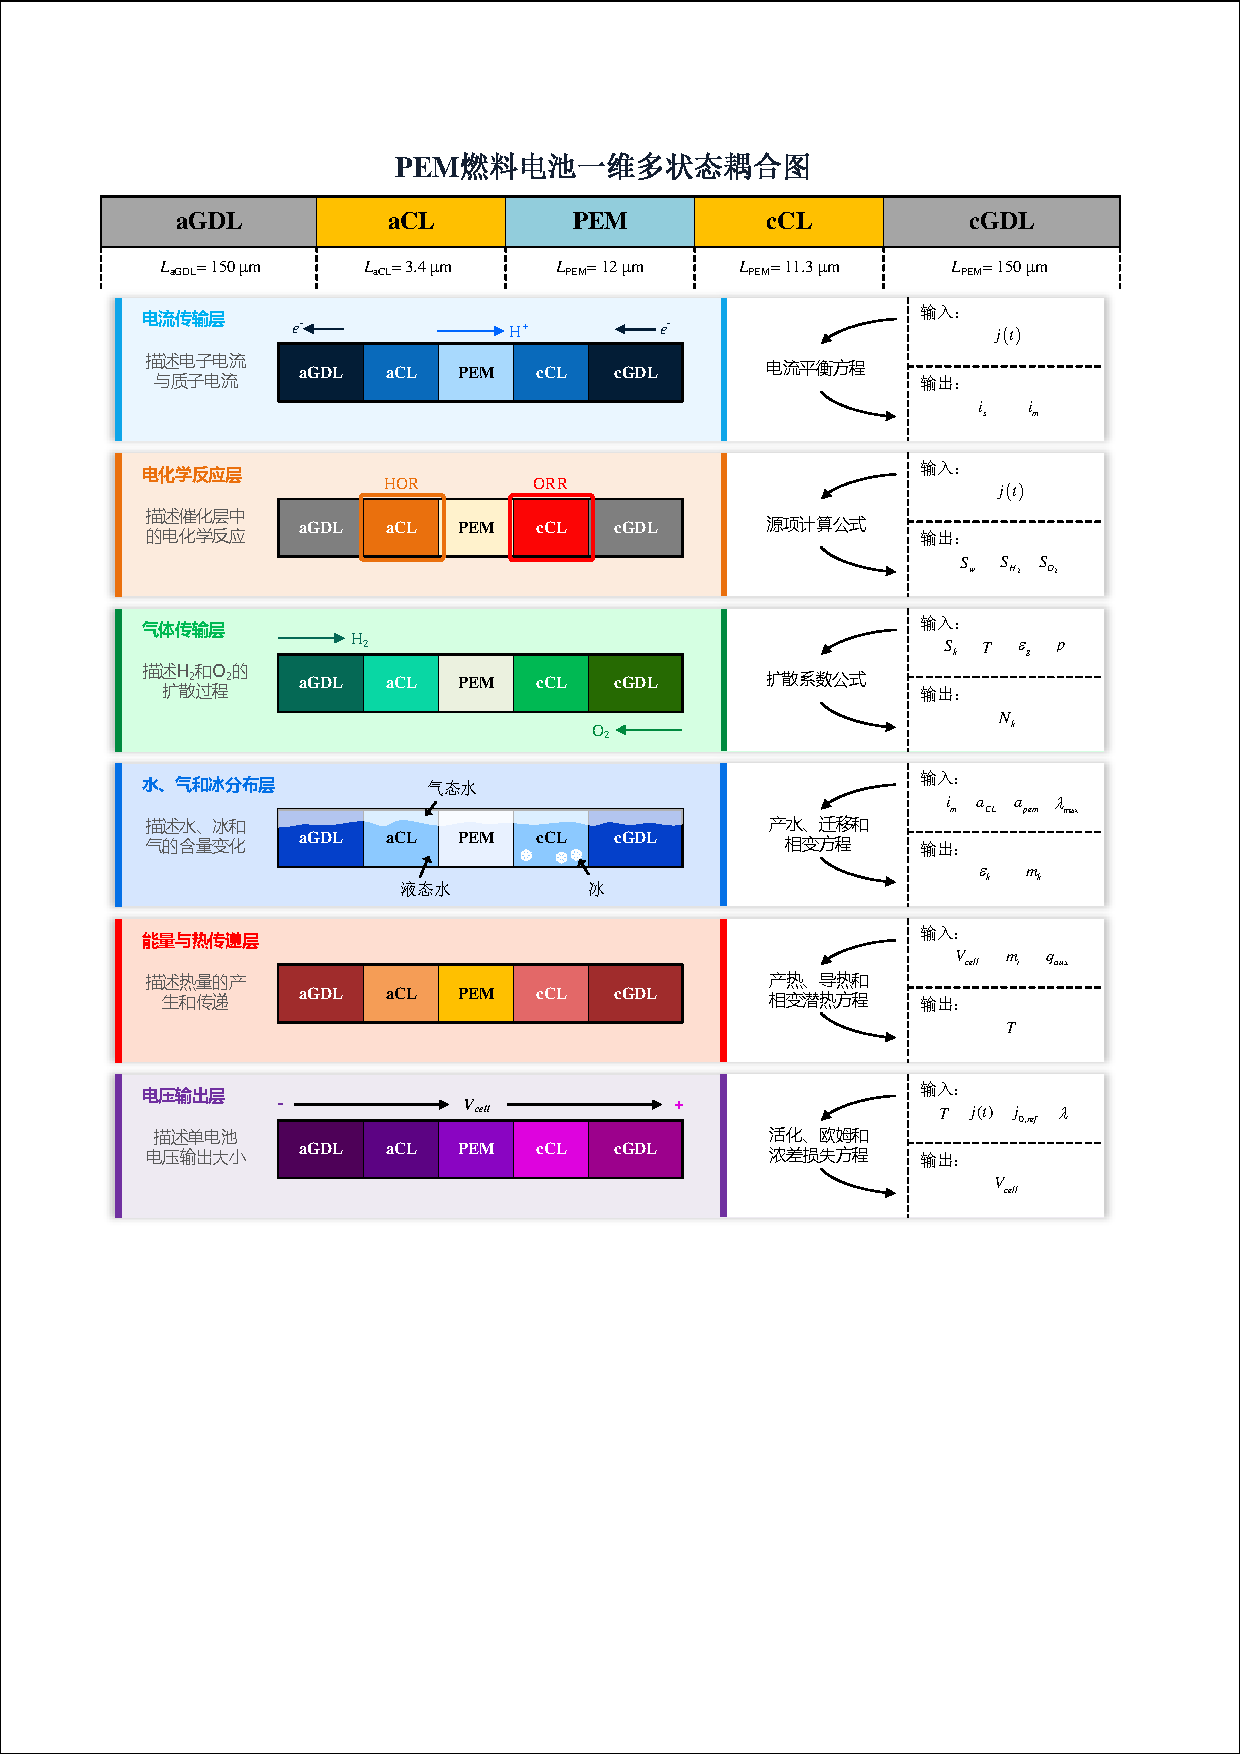
\includegraphics[width=0.95\linewidth,height=0.78\textheight,keepaspectratio,trim=40bp 245bp 40bp 40bp,clip]{figures/problem1_model.pdf}
  \caption{问题一单电池一维多物理场耦合示意图}
  \label{fig:p1_coupling}
\end{figure}

\subsection{控制方程}

\subsubsection{气体守恒方程}

氢气与氧气在气体扩散层及催化层中满足
\begin{equation}
  \frac{\partial(\varepsilon_g c_k)}{\partial t}
  =\frac{\partial}{\partial x}\!\left(D_{k,\mathrm{eff}}\frac{\partial c_k}{\partial x}\right)+S_k,
  \qquad k=\mathrm{H_2},\mathrm{O_2},
  \label{eq:gas}
\end{equation}
源项仅出现在对应催化层中，其余区域取零：
\begin{equation}
  S_{\mathrm{H_2}}=-\frac{j}{2FL_{\mathrm{aCL}}},\quad x\in\Omega_{\mathrm{aCL}};
  \qquad
  S_{\mathrm{O_2}}=-\frac{j}{4FL_{\mathrm{cCL}}},\quad x\in\Omega_{\mathrm{cCL}}.
  \label{eq:gassource}
\end{equation}
有效扩散系数采用 Bruggeman 孔隙率修正，并以扣除液态水与冰体积后的动态气相孔隙率计算。离散时显式保留孔隙率变化引起的气体稀释与浓缩效应，具体闭合关系及有限体积离散式见附录\ref{app:p1-details}。

\subsubsection{总水守恒方程与水通量}

总水量仍采用统一描述，其守恒方程为
\begin{equation}
  \frac{\partial m_w}{\partial t}=-\frac{\partial N_w}{\partial x}+S_w,
  \qquad
  S_w=\frac{M_w j}{2FL_{\mathrm{cCL}}},\quad x\in\Omega_{\mathrm{cCL}},
  \label{eq:water}
\end{equation}
水通量由三部分叠加：
\begin{equation}
  N_w=N_{\mathrm{vap}}+N_{\mathrm{liq}}+N_{\mathrm{eod}}.
  \label{eq:nw}
\end{equation}

其中，水蒸气在多孔层内扩散、在膜内以吸附态迁移；液态水在毛细压力梯度下排出；质子迁移产生电渗拖曳。三部分通量的具体表达、CL|PEM 界面导通关系及冰堵后的渗透率修正见附录\ref{app:p1-details}。

\subsubsection{水的三态相平衡与冰体积分数}

三态分配时先从总水量中扣除离聚物结合水，再将孔隙水依次分为冰、饱和水蒸气与液态水。具体反演关系见附录\ref{app:p1-details}。冰体积分数定义为网格单元内冰相体积与该网格单元总体积之比。由于 $m_i$ 为单位网格单元体积内的冰质量，故
\begin{equation}
  \varepsilon_{\mathrm{ice}}=\frac{V_{\mathrm{ice}}}{V_{\mathrm{cv}}}
  =\frac{m_i}{\rho_{\mathrm{ice}}}=\varepsilon_i,
  \label{eq:icevf}
\end{equation}
即以网格单元总体积为基准。

\subsubsection{液态水/冰相变控制方程}

冰作为独立状态量，其守恒方程（即相变控制方程）为
\begin{equation}
  \frac{\partial m_i}{\partial t}=R_{\mathrm{frz}}-R_{\mathrm{mlt}},
  \label{eq:iceeq}
\end{equation}
相变速率采用以冰点 $T_f=273.15~\mathrm{K}$ 为判据的分段关系~\cite{mao2007multiphase}：
\begin{equation}
  R_{\mathrm{frz}}=k_{\mathrm{frz}}\,\rho_l\varepsilon_0 s_l=k_{\mathrm{frz}}\,m_l,
  \quad T\le T_f;
  \qquad
  R_{\mathrm{mlt}}=k_{\mathrm{mlt}}\,\rho_{\mathrm{ice}}\varepsilon_i=k_{\mathrm{mlt}}\,m_i,
  \quad T>T_f.
  \label{eq:phase}
\end{equation}
冰量的物理约束见附录\ref{app:p1-details}。

\subsubsection{阴极催化层离聚物水合动力学}

停机吹扫后催化层比质子交换膜更干，冷启动初期反应生成的水优先水合离聚物，达到低温上限后才进入孔隙并参与排水与结冰。以 $\lambda_{\mathrm{cCL}}$ 描述 cCL 离聚物平均含水量，其动力学方程为
\begin{equation}
  \frac{\mathrm{d}\lambda_{\mathrm{cCL}}}{\mathrm{d}t}
  =\min\!\left\{
    \frac{\lambda_{\mathrm{sat}}(T)-\lambda_{\mathrm{cCL}}}{\tau_{\mathrm{hyd}}},~
    \frac{\lambda_{\mathrm{avail}}-\lambda_{\mathrm{cCL}}}{\tau_{\mathrm{hyd}}}
    +\frac{\dot{m}_{w,\mathrm{rxn}}}{\varepsilon_{\mathrm{ion}}\rho_{\mathrm{ion}}M_w/\mathrm{EW}}
  \right\},
  \label{eq:hyd}
\end{equation}
式中第二项限制水合速率不超过实际可供水量与反应生成水之和。$\lambda_{\mathrm{avail}}$、$\dot m_{w,\mathrm{rxn}}$ 及低温最大非冻结含水量 $\lambda_{\mathrm{sat}}$ 的表达式见附录\ref{app:p1-details}；其中 $\lambda_{\mathrm{sat}}$ 为物性关系，而非新增拟合参数。

\subsubsection{能量守恒方程}

温度场满足
\begin{equation}
  (\rho c_p)_{\mathrm{eff}}\frac{\partial T}{\partial t}
  =\frac{\partial}{\partial x}\!\left(k_{\mathrm{eff}}\frac{\partial T}{\partial x}\right)
  +\dot q_{\mathrm{gen}}+\dot q_{\mathrm{ph}}+\dot q_{\mathrm{aux}},
  \label{eq:energy}
\end{equation}
其中电化学产热仍按热中性电压统一计算
\begin{equation}
  \dot q_{\mathrm{gen}}=\frac{j\,(E_{\mathrm{th}}-V_{\mathrm{cell}})}{L},
  \qquad E_{\mathrm{th}}=1.48~\mathrm{V},
  \label{eq:qgen}
\end{equation}
相变潜热源项为
\begin{equation}
  \dot q_{\mathrm{ph}}=h_{\mathrm{sf}}\frac{\partial m_i}{\partial t},
  \qquad h_{\mathrm{sf}}=333600~\mathrm{J\cdot kg^{-1}},
  \label{eq:qph}
\end{equation}
因而冻结（$\partial m_i/\partial t>0$）放热、融化（$\partial m_i/\partial t<0$）吸热；自冷启动工况下 $\dot q_{\mathrm{aux}}=0$。等效体积热容采用体积分数加权，等效导热系数采用串联热阻计算，具体关系见附录\ref{app:p1-details}。

\subsubsection{单电池电压与三项极化损失}

单电池电压由可逆电压减去三项极化损失得到。活化损失沿用常温参考模型中的表达，但交换电流密度需同时考虑离聚物水合程度与冰覆盖程度：
\begin{equation}
  j_{0,\mathrm{eff}}=j_0(T)\,f_{\mathrm{hyd}}\,f_{\mathrm{ice}},
  \qquad
  j_0(T)=j_{0,\mathrm{ref}}\exp\!\left[-\frac{E_a}{R}\!\left(\frac{1}{T}-\frac{1}{298.15}\right)\right],
  \label{eq:j0eff}
\end{equation}
\begin{equation}
  f_{\mathrm{ice}}=\bigl(1-s_{i,\mathrm{cCL}}\bigr)^{\gamma_{\mathrm{ice}}},
  \qquad
  f_{\mathrm{hyd}}=\left(\frac{\lambda_{\mathrm{cCL}}}{\lambda_{\mathrm{hyd,ref}}}\right)^{m_{\mathrm{hyd}}},
  \qquad \lambda_{\mathrm{hyd,ref}}=1.
  \label{eq:fhyd}
\end{equation}
式（\ref{eq:fhyd}）中 $f_{\mathrm{ice}}$ 表示冰对催化层有效反应面积的修正；$f_{\mathrm{hyd}}$ 随离聚物含水量增加而增大。参考含水量固定为初始 cCL 含水量，不参与标定。

欧姆损失在常温模型只计膜电阻的基础上，补充两个催化层离聚物内的质子传导损失：
\begin{equation}
  \eta_{\mathrm{ohm}}
  =\int_{\mathrm{pem}}\frac{i_m}{\kappa_{\mathrm{pem}}}\,\mathrm{d}x
  +\int_{\mathrm{aCL}}\frac{i_m}{\kappa_{\mathrm{aCL}}}\,\mathrm{d}x
  +\int_{\mathrm{cCL}}\frac{i_m}{\kappa_{\mathrm{cCL}}}\,\mathrm{d}x
  +jR_c,
  \label{eq:etaohm}
\end{equation}
膜与催化层质子电导率的含水量关联式见附录\ref{app:p1-details}，其中催化层电导率采用 Bruggeman 修正。由于 $\lambda_{\mathrm{cCL}}$ 在启动初期较低，该项给出冷启动前期显著的额外欧姆损失，并随产水水合自然衰减。

浓差损失采用常温参考模型中的浓差极化关系计算，极限电流密度由 cCL 与 cGDL 沿厚度方向的串联扩散阻力确定，具体表达式见附录\ref{app:p1-details}。

\subsection{初始条件与边界条件}

设启动初始温度为 $T_0$，并取 $T_{\mathrm{amb}}=T_0$。吹扫后多孔层内无液态水和冰，膜内保留少量结合水，催化层离聚物初始含水量低于膜含水量。阳极与阴极外侧分别接干氢气和干空气，水蒸气采用干气道零浓度边界；两侧按双极板导热热阻与环境对流热阻串联散热；各功能层交界面满足相应通量连续条件。完整的初始条件与边界条件列于附录\ref{app:p1-details}。

\subsection{参数取值与标定}

几何尺寸、层厚、材料物性、电化学常数和冰物性等参数直接取自附件1 与备注1。计算采用 \texttt{Code\_ICE\_F} 的参数组：$E_a=67000~\mathrm{J\cdot mol^{-1}}$ 与 $\gamma_{\mathrm{ice}}=3.5$ 取自原始参数，$k_{\mathrm{frz}}=0.4~\mathrm{s^{-1}}$ 为固定值；利用两个低温工况的电压曲线标定 $j_{0,\mathrm{ref}}$、$m_{\mathrm{hyd}}$、催化层电阻缩放系数和 $\tau_{\mathrm{hyd}}$。各参数取值与来源见\Cref{tab:p1_params}。

\begin{table}[htbp]
  \centering\small
  \caption{冷启动模型主要参数的取值与来源}
  \label{tab:p1_params}
  \begin{tabularx}{0.90\linewidth}{>{$}p{0.24\linewidth}<{$}>{\centering\arraybackslash}p{0.30\linewidth}>{\centering\arraybackslash}X}
    \toprule
    \multicolumn{1}{l}{参数} & 取值 & 来源\\
    \midrule
    \rho_{\mathrm{ice}} & $920~\mathrm{kg\cdot m^{-3}}$ & 附件1\\
    h_{\mathrm{sf}} & $333600~\mathrm{J\cdot kg^{-1}}$ & 附件1\\
    \varepsilon_{\mathrm{ion}} & $0.3$ & 附件1\\
    \lambda_0,\ \lambda_{\mathrm{cCL},0} & $3,\ 1$ & 附件1与模型设定\\
    k_{\mathrm{frz}} & $0.4~\mathrm{s^{-1}}$ & 固定值\\
    k_{\mathrm{mlt}} & $0~\mathrm{s^{-1}}$ & 模型设定\\
    \gamma_{\mathrm{ice}} & $3.5$ & 附件1\\
    \tau_{\mathrm{hyd}} & $40~\mathrm{s}$ & 两个低温工况标定\\
    m_{\mathrm{hyd}} & $1.70$ & 两个低温工况标定\\
    \mathrm{CL\ resistance\ scale} & $0.66$ & 两个低温工况标定\\
    j_{0,\mathrm{ref}} & $0.28~\mathrm{A\cdot m^{-2}}$ & 两个低温工况标定\\
    E_a & $67000~\mathrm{J\cdot mol^{-1}}$ & 题目式(40)\\
    \zeta & $30$ & 模型设定\\
    \bottomrule
  \end{tabularx}
\end{table}

\subsection{数值求解}

控制方程（\ref{eq:gas}）、（\ref{eq:water}）、（\ref{eq:iceeq}）、（\ref{eq:hyd}）与（\ref{eq:energy}）连同式（\ref{eq:j0eff}）--（\ref{eq:jlim}）的代数关系构成指标为 $1$ 的半显式微分代数方程组，空间离散后得到 $215$ 维刚性常微分方程组，采用 MATLAB R2024b 的变阶刚性求解器 \texttt{ode15s} 求解，主要设置与步骤如下：

\begin{enumerate}
  \item 读取附件2 中对应工况的电流密度序列，以线性插值构造输入 $j(t)$；
  \item 按式（\ref{eq:init}）装配初始状态，并检验冰量、孔隙率与含水量的物理可行性；
  \item 设置 $\mathrm{RelTol}=10^{-6}$、$\mathrm{AbsTol}=10^{-8}$、最大步长 $\mathrm{MaxStep}=0.01~\mathrm{s}$，并对气体浓度、总水量、冰量与 $\lambda_{\mathrm{cCL}}$ 启用非负约束，避免 Newton 试探值破坏物理意义；
  \item 以附件2 的采样时刻为输出时刻积分至 $36.6~\mathrm{s}$；
  \item 求解后重算代数输出，并检查总水守恒、能量守恒、冰量上界与电流是否低于极限电流。
\end{enumerate}

\subsection{求解结果与分析}
\label{sec:model1_result}

\subsubsection{与实验数据的对比}

\Cref{fig:p1_verify_T20} 与\Cref{fig:p1_verify_T25} 分别给出两个工况下加载电流密度、单电池电压、平均温度与最大冰体积分数的时间历程，\Cref{tab:p1_T20}、\Cref{tab:p1_T25} 给出题目表1、表2 所要求的八个时刻的结果。相对误差按题目要求定义为
\begin{equation}
  \varepsilon_X=\frac{|X_{\mathrm{sim}}-X_{\mathrm{exp}}|}{|X_{\mathrm{exp}}|}\times100\%,
  \label{eq:relerr}
\end{equation}
其中 $X$ 为单电池电压或平均温度（温度以摄氏度的绝对值归一化）。

\begin{figure}[H]
  \centering
  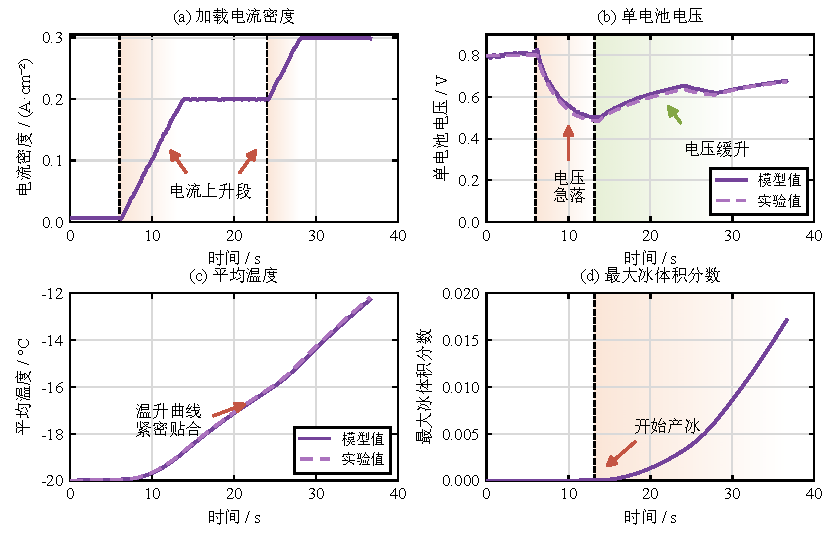
\includegraphics[width=0.82\linewidth]{figures/p1_f_verify_T20.pdf}
  \caption{$-20~^{\circ}\mathrm{C}$ 工况模型与实验对比}
  \label{fig:p1_verify_T20}
\end{figure}

\begin{table}[H]
  \centering\small
  \caption{一维单电池瞬态自冷启动模型预测与实验验证结果（$-20~^{\circ}\mathrm{C}$）}
  \label{tab:p1_T20}
  \begin{tabularx}{\linewidth}{c*{7}{>{\centering\arraybackslash}X}}
    \toprule
    时间/s & 实验电压/V & 模型电压/V & 电压相对误差/\% & 实验温度/$^{\circ}\mathrm{C}$ & 模型温度/$^{\circ}\mathrm{C}$ & 温度相对误差/\% & 模型最大冰体积分数\\
    \midrule
    0  & 0.799 & 0.7962 & 0.35 & $-20.00$ & $-20.000$ & 0.00 & 0\\
    5  & 0.801 & 0.8058 & 0.60 & $-19.96$ & $-19.966$ & 0.03 & 0\\
    10 & 0.538 & 0.5587 & 3.84 & $-19.65$ & $-19.675$ & 0.13 & 0\\
    15 & 0.521 & 0.5313 & 1.98 & $-18.41$ & $-18.445$ & 0.19 & 0.0001\\
    20 & 0.599 & 0.6144 & 2.57 & $-17.08$ & $-17.118$ & 0.22 & 0.0013\\
    25 & 0.626 & 0.6437 & 2.83 & $-15.90$ & $-15.957$ & 0.36 & 0.0038\\
    30 & 0.633 & 0.6361 & 0.48 & $-14.27$ & $-14.353$ & 0.58 & 0.0086\\
    35 & 0.666 & 0.6693 & 0.50 & $-12.67$ & $-12.748$ & 0.62 & 0.0149\\
    \bottomrule
  \end{tabularx}
\end{table}

\begin{figure}[H]
  \centering
  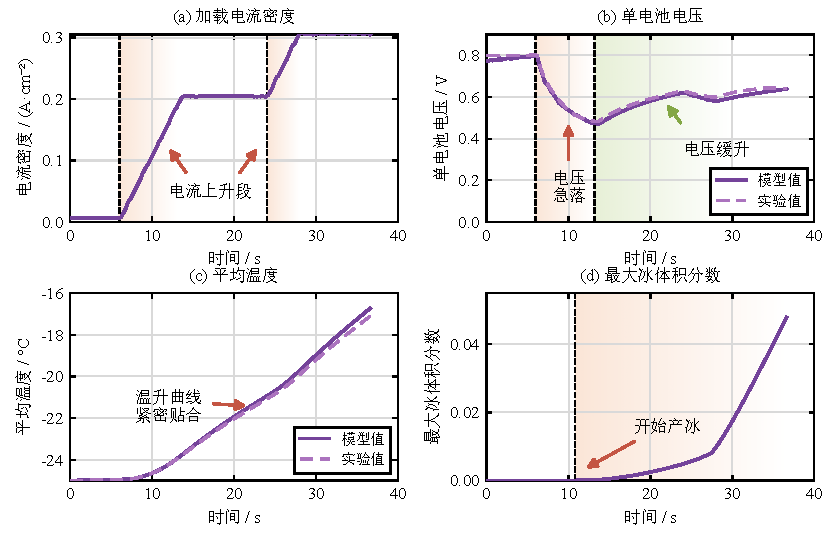
\includegraphics[width=0.82\linewidth]{figures/p1_f_verify_T25.pdf}
  \caption{$-25~^{\circ}\mathrm{C}$ 工况模型与实验对比}
  \label{fig:p1_verify_T25}
\end{figure}

\begin{table}[H]
  \centering\small
  \caption{一维单电池瞬态自冷启动模型预测与实验验证结果（$-25~^{\circ}\mathrm{C}$）}
  \label{tab:p1_T25}
  \begin{tabularx}{\linewidth}{c*{7}{>{\centering\arraybackslash}X}}
    \toprule
    时间/s & 实验电压/V & 模型电压/V & 电压相对误差/\% & 实验温度/$^{\circ}\mathrm{C}$ & 模型温度/$^{\circ}\mathrm{C}$ & 温度相对误差/\% & 模型最大冰体积分数\\
    \midrule
    0  & 0.799 & 0.7738 & 3.15 & $-25.00$ & $-25.000$ & 0.00 & 0\\
    5  & 0.800 & 0.7944 & 0.70 & $-24.96$ & $-24.963$ & 0.01 & 0\\
    10 & 0.537 & 0.5356 & 0.27 & $-24.65$ & $-24.644$ & 0.02 & 0\\
    15 & 0.518 & 0.5005 & 3.39 & $-23.38$ & $-23.339$ & 0.18 & 0.0005\\
    20 & 0.592 & 0.5813 & 1.80 & $-22.03$ & $-21.933$ & 0.44 & 0.0025\\
    25 & 0.618 & 0.6076 & 1.69 & $-20.85$ & $-20.695$ & 0.74 & 0.0056\\
    30 & 0.621 & 0.5972 & 3.82 & $-19.20$ & $-18.967$ & 1.22 & 0.0174\\
    35 & 0.644 & 0.6296 & 2.24 & $-17.59$ & $-17.243$ & 1.97 & 0.0402\\
    \bottomrule
  \end{tabularx}
\end{table}

\Cref{tab:p1_summary} 汇总两个工况的整体误差与冰量输出。两工况全时段的电压均方根误差分别为 $0.01329~\mathrm{V}$ 与 $0.01438~\mathrm{V}$，温度均方根误差分别为 $0.050~^{\circ}\mathrm{C}$ 与 $0.160~^{\circ}\mathrm{C}$。模型在两个工况下均再现了电压快速下降后回升、温度持续上升的总体变化趋势。

\begin{table}[htbp]
  \centering\small
  \caption{两工况整体误差与冰量输出汇总}
  \label{tab:p1_summary}
  \begin{tabularx}{0.86\linewidth}{>{\raggedright\arraybackslash}Xcc}
    \toprule
    指标 & $-20~^{\circ}\mathrm{C}$ & $-25~^{\circ}\mathrm{C}$\\
    \midrule
    电压 RMSE / V                     & 0.01329        & 0.01438\\
    温度 RMSE / $^{\circ}\mathrm{C}$  & 0.050         & 0.160\\
    八个报告时刻最大电压相对误差 / \% & 3.84（$t=10~\mathrm{s}$） & 3.82（$t=30~\mathrm{s}$）\\
    $36.6~\mathrm{s}$ 电压 / V        & 0.6785        & 0.6388\\
    $36.6~\mathrm{s}$ 平均温度 / $^{\circ}\mathrm{C}$ & $-12.27$ & $-16.73$\\
    $35~\mathrm{s}$ 最大冰体积分数    & 0.0149        & 0.0402\\
    全时段最大冰体积分数              & 0.0171        & 0.0479\\
    $36.6~\mathrm{s}$ 冰面密度 / $\mathrm{kg\cdot m^{-2}}$ & $1.78\times10^{-4}$ & $3.09\times10^{-4}$\\
    $36.6~\mathrm{s}$ cCL 孔隙冰饱和度 & 0.0407 & 0.0706\\
    \bottomrule
  \end{tabularx}
\end{table}

\subsubsection{冰的分布与演化}

\Cref{fig:p1_ice_profile} 展示 $10$--$35~\mathrm{s}$ 内阴极催化层（cCL）与阴极气体扩散层（cGDL）的冰体积分数分布；横轴为多孔介质网格单元编号，颜色表示时刻。两个工况的冰主要分布在 cCL，cGDL 中未出现明显积冰。$35~\mathrm{s}$ 时，$-20~^{\circ}\mathrm{C}$ 与 $-25~^{\circ}\mathrm{C}$ 工况的峰值分别约为 $0.0149$ 与 $0.0402$。这一分布是模型对内部状态的预测，而非冰量实测结果。

\begin{figure}[H]
  \centering
  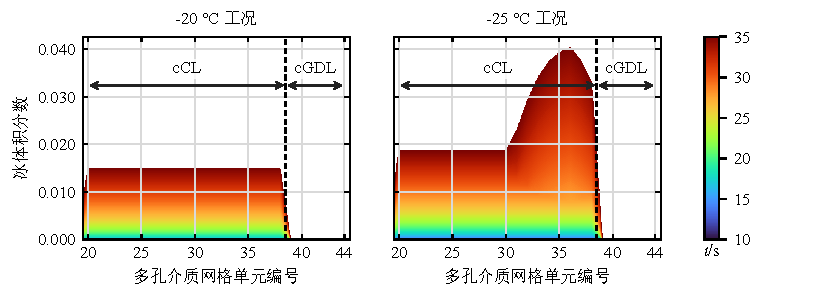
\includegraphics[width=14cm]{figures/p1_f_ice_profiles_timecolor.pdf}
  \caption{$10$--$35~\mathrm{s}$ 内阴极侧冰体积分数的空间分布与演化}
  \label{fig:p1_ice_profile}
\end{figure}

综合\Cref{fig:p1_verify_T20}、\Cref{fig:p1_verify_T25}与\Cref{tab:p1_summary} 可见，模型能够同时再现两个低温工况下电压先快速下降后逐步回升、温度持续升高的实验变化趋势。两工况的电压均方根误差分别为 $0.01329~\mathrm{V}$ 和 $0.01438~\mathrm{V}$，温度均方根误差分别为 $0.050~^{\circ}\mathrm{C}$ 和 $0.160~^{\circ}\mathrm{C}$，说明所建冷启动模型与附件2实验数据具有较好的一致性，可作为后续启动策略优化的基础。由于附件2未提供冰量实测数据，本文给出的冰分布和冰体积分数仅作为模型状态量输出，不将其作为标定精度的独立验证依据。

\subsubsection{电压损失的分解与机理检验}

\Cref{fig:p1_loss} 与\Cref{tab:p1_loss} 给出各项电压与损失的时间历程。可以发现：

\begin{enumerate}
  \item 可逆电压在全程内的变化约为 $0.007~\mathrm{V}$，浓差损失始终小于 $7\times10^{-5}~\mathrm{V}$；本工况的电压变化主要由活化损失和欧姆损失决定。
  \item 快速升流阶段两项损失均显著增加。以 $-20~^{\circ}\mathrm{C}$ 为例，$10~\mathrm{s}$ 时活化损失和欧姆损失分别为 $0.5372~\mathrm{V}$ 和 $0.1625~\mathrm{V}$；随后水合使欧姆损失逐渐减小，$35~\mathrm{s}$ 时降为 $0.1007~\mathrm{V}$。
  \item $36.6~\mathrm{s}$ 时，$\lambda_{\mathrm{cCL}}$ 分别达到 $4.74$ 和 $4.33$，冰覆盖面积因子分别为 $0.865$ 和 $0.774$。这些内部状态用于解释模型电压响应，但缺少独立实测，不单独作为模型精度的证据。
\end{enumerate}

\begin{figure}[H]
  \centering
  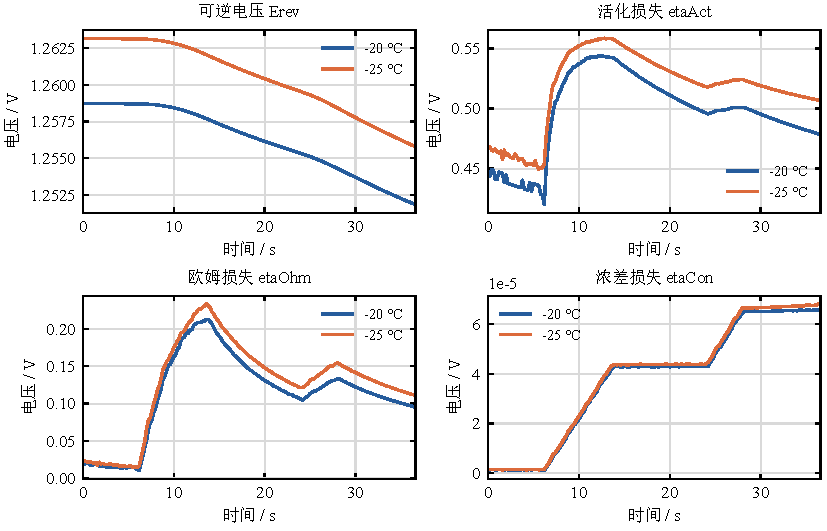
\includegraphics[width=0.82\linewidth]{figures/p1_f_loss.pdf}
  \caption{可逆电压与三项极化损失的时间历程}
  \label{fig:p1_loss}
\end{figure}

\begin{table}[H]
  \centering\small
  \caption{典型时刻的电压损失分解（单位：V）}
  \label{tab:p1_loss}
  \begin{tabularx}{0.86\linewidth}{cc*{5}{>{\centering\arraybackslash}X}}
    \toprule
    时刻/s & 工况 & $E_{\mathrm{rev}}$ & $\eta_{\mathrm{act}}$ & $\eta_{\mathrm{ohm}}$ & $\eta_{\mathrm{con}}$ & $V_{\mathrm{cell}}$\\
    \midrule
    0  & $-20~^{\circ}\mathrm{C}$ & 1.2587 & 0.4438 & 0.0187 & $<10^{-5}$ & 0.7962\\
    10 & $-20~^{\circ}\mathrm{C}$ & 1.2584 & 0.5372 & 0.1625 & 0.00002 & 0.5587\\
    20 & $-20~^{\circ}\mathrm{C}$ & 1.2562 & 0.5109 & 0.1308 & 0.00004 & 0.6144\\
    35 & $-20~^{\circ}\mathrm{C}$ & 1.2523 & 0.4821 & 0.1007 & 0.00007 & 0.6693\\
    \midrule
    0  & $-25~^{\circ}\mathrm{C}$ & 1.2632 & 0.4665 & 0.0228 & $<10^{-5}$ & 0.7738\\
    10 & $-25~^{\circ}\mathrm{C}$ & 1.2628 & 0.5522 & 0.1750 & 0.00002 & 0.5356\\
    20 & $-25~^{\circ}\mathrm{C}$ & 1.2604 & 0.5310 & 0.1480 & 0.00004 & 0.5813\\
    35 & $-25~^{\circ}\mathrm{C}$ & 1.2562 & 0.5093 & 0.1173 & 0.00007 & 0.6296\\
    \bottomrule
  \end{tabularx}
\end{table}

两个工况的平均温度曲线均与实验趋势相符，表明模型给出的热响应可用于冷启动策略的初步分析。

\subsection{模型检验}
\label{sec:model1_check}

\subsubsection{守恒性与数值收敛性}

本次按 \texttt{Code\_ICE\_F} 默认求解设置，以最大步长 $0.01~\mathrm{s}$ 对两个工况重新积分；电压、温度和冰量图均直接由同一组求解状态生成。更细步长的独立收敛性数据未在本次重绘中更新，故不沿用旧版数值。

\subsubsection{参数固定性与可辨识性}

冰覆盖指数 $\gamma_{\mathrm{ice}}=3.5$ 与冻结速率系数 $k_{\mathrm{frz}}=0.4~\mathrm{s^{-1}}$ 在本次计算中固定，未由附件2的电压数据重新辨识。由于缺少冰量实测，模型预测的冰状态仍需后续实验检验。

膜与阴极催化层的水合变化及冰覆盖对有效反应面积的影响见\Cref{fig:p1_hydration}。
\begin{figure}[H]
  \centering
  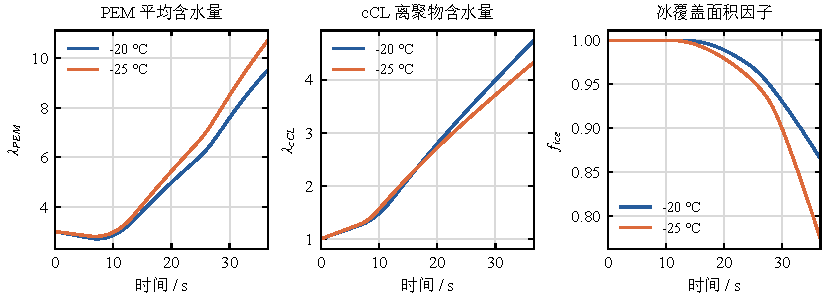
\includegraphics[width=0.86\linewidth]{figures/p1_f_hydration.pdf}
  \caption{PEM 与 cCL 离聚物含水量及水合、冰覆盖面积因子}
  \label{fig:p1_hydration}
\end{figure}

\subsubsection{误差来源与预测能力评价}

两个工况在报告时刻的电压相对误差均不超过 $3.84\%$，温度曲线也跟随实验持续升高。$-25~^{\circ}\mathrm{C}$ 工况的温度 RMSE 为 $0.160~^{\circ}\mathrm{C}$，高于 $-20~^{\circ}\mathrm{C}$ 工况的 $0.050~^{\circ}\mathrm{C}$；该温度依赖性的误差是模型后续改进的重点。综合来看，模型能够为后续冷启动策略研究提供经两个低温实验工况检验的基础，但冰的空间分布仍是待验证预测。

\section{问题二模型的建立与求解}
\label{sec:model2}

问题二将问题一的一维单电池模型扩展到五片串联电堆，并在单位面积累积电荷、单片电压、冰量与电流密度的共同约束下，分别对恒流加载、线性升载和分段阶梯加载三种电流曲线进行优化。三种策略均以五片单电池全部达到启动温度所需时间最短为目标，并在统一的物理参数、数值网格和约束条件下比较其冷启动性能；随后利用优化后的加载策略确定电堆能够实现自冷启动的最低初始温度。

\subsection{五片电堆状态与热耦合}

第 $k$ 片单电池仍保留问题一中的温度、反应气体、水和冰以及阴极催化层离聚物含水量等全部离散状态，记为
\begin{equation}
  \bm{x}_k=
  \left[\bm{T}_k,\bm{c}_{\mathrm{H_2},k},
  \bm{c}_{\mathrm{O_2},k},\bm{m}_{w,k},
  \bm{m}_{i,k},\bm{\lambda}_{\mathrm{cCL},k}\right]^{\mathrm T}.
\end{equation}
五片电池施加相同的电流密度，电堆状态在五组单片状态之外增加单位面积累积电荷 $q_{\mathrm{use}}$ 以及左右端板温度 $T_{e,L}$、$T_{e,R}$：
\begin{equation}
  \bm{X}=\left[\bm{x}_1^{\mathrm T},\ldots,\bm{x}_5^{\mathrm T},
  q_{\mathrm{use}},T_{e,L},T_{e,R}\right]^{\mathrm T},
  \qquad
  \frac{\mathrm d q_{\mathrm{use}}}{\mathrm dt}=j(t),
  \quad q_{\mathrm{use}}(0)=0.
  \label{eq:q2-charge}
\end{equation}
相邻单片之间采用守恒的面热通量耦合。令 $\bar T_k$ 为第 $k$ 片的厚度加权平均温度，则第 $k$ 片流向第 $k+1$ 片的热通量为
\begin{equation}
  q''_{k,k+1}=G''_{\mathrm{cell}}(\bar T_k-\bar T_{k+1}),
  \qquad
  G''_{\mathrm{cell}}=\frac{1}{R''_{\mathrm{MEA}}+R''_{\mathrm{BP}}},
  \label{eq:q2-intercell-heat}
\end{equation}
其中
\begin{equation}
  R''_{\mathrm{MEA}}=\sum_{r}\frac{L_r}{k_r},
  \qquad
  R''_{\mathrm{BP}}=\frac{L_{\mathrm{BP}}}{k_{\mathrm{BP}}}.
\end{equation}
同一个 $q''_{k,k+1}$ 分别作为两片电池的流出项和流入项，因此内部换热在电堆总能量方程中严格抵消。五片堆共有六块双极板。为避免把片间共享双极板重复计入热容，五片单电池对应的双极板热容倍率取
\begin{equation}
  \bm{\chi}_{\mathrm{BP}}=(0.75,0.50,0.50,0.50,0.75)^{\mathrm T},
\end{equation}
其总量恰好对应六块双极板。

两侧端板不与端部单片强制同温，而是作为独立热节点。以左端板为例，其能量平衡写为
\begin{equation}
  C''_{e}\frac{\mathrm d T_{e,L}}{\mathrm dt}
  =\frac{\bar T_1-T_{e,L}}{R''_{c-e}}
  -\frac{T_{e,L}-T_{\mathrm{amb}}}{R''_{e-a}},
  \qquad
  C''_{e}=\rho_e c_{p,e}L_e,
  \label{eq:q2-endplate}
\end{equation}
右端板具有同样的形式。这里 $R''_{c-e}$ 包含半个膜电极、一个双极板和半个端板的串联热阻，$R''_{e-a}$ 包含半个端板的导热热阻与外表面对流热阻。该处理允许启动时端板仍明显低于 $0~^{\circ}\mathrm{C}$，同时不迫使端部单片与端板同步升温。

% ===== 恒流加载策略（结果包：2 s 升流后保持平台电流） =====
% 恒流协议经 2 s 短升流建立平台电流：物理上对应文献推荐的缓启动方式
% （避免干膜电压下冲/反极与快速冰堵），数值上避免准静态电压方程的
% t=0 初值越界（阶跃恒流会在 t=0 即触发 0.30 V 下限事件）。
% 真正的 t=0 阶跃恒流对照见相邻结果包 Q2_True_Constant_Baseline。

\subsection{恒流加载策略}
\label{subsec:q2-cc}

恒流加载是三种候选加载方式中最简单的一种：电流在短暂建立后保持不变，整个启动过程只由平台电流一个设计参数控制。下面依次给出其优化模型、求解方法、仿真设置与优化结果，并基于优化后的固定加载曲线确定电堆的最低自启动初温。

\subsubsection{优化模型}
\label{subsec:q2-cc-model}

恒流加载曲线由初始电流密度 $j_0$、升流时间 $\tau_r$ 与平台电流密度 $j_p$ 刻画，其形式为
\begin{equation}
  j(t;j_p)=\min\left\{j_0+\frac{j_p-j_0}{\tau_r}\,t,\ j_p\right\},
  \qquad j_0=0.0200~\mathrm{A\,cm^{-2}},\quad \tau_r=2~\mathrm{s}.
  \label{eq:q2-cc-current}
\end{equation}
恒流加载并不意味着在 $t=0$ 时刻阶跃建立电流。冷启动初始时刻膜处于低水合、高阻抗状态，若瞬间施加平台电流，电渗拖拽将在亚秒级时间尺度内进一步使膜脱水、欧姆阻抗升高，单片电压出现瞬时下冲，严重时甚至发生反极~\cite{hussaini2009transients,gao2022reverse}；同时阴极产水速率突变，大量生成水在膜尚未充分水合时冻结，加速催化层冰堵，这正是恒流启动的主要风险~\cite{yao2020failure}。因此文献普遍推荐以线性或阶梯方式逐渐建立电流，使产热与产水的时序相互匹配~\cite{jiang2010ramping,luo2018coldstart}。据此，本文的恒流协议从 $0.02~\mathrm{A\,cm^{-2}}$ 起、经 $\tau_r=2~\mathrm{s}$ 线性升至平台电流后保持恒流。这一短升流段同时也是模型层面的必要处理：本文单片电压方程为不含双电层电容的准静态形式 $V=E_{\mathrm{rev}}-\eta_{\mathrm{act}}-\eta_{\mathrm{ohm}}-\eta_{\mathrm{con}}$，阶跃电流会使低温干膜上的欧姆与活化过电位瞬时建立，初始电压在 $t=0$ 处即低于 $0.30~\mathrm{V}$ 下限、触发失效事件而无法起步，与真实电子负载有限的电流上升速率也不相符；升流段电荷按梯形计入累计电荷约束。固定 $j_0$ 与 $\tau_r$ 后，恒流协议退化为仅由平台电流 $j_p$ 决定的单参数加载方式，将其归一化为
\begin{equation}
  x=\frac{j_p-0.02}{0.48}\in[0,1],
  \qquad j_p=0.02+0.48\,x.
  \label{eq:q2-cc-decode}
\end{equation}
目标函数与约束形式与线性升载策略相同，即式\eqref{eq:q2-objective}定义的启动时间最小化问题，只是搜索域收缩为一维；本结果包的孔隙占用阈值取 $0.99$（见\Cref{tab:q2-cc-settings}）。

固定参考组取平台电流 $j_p=0.259937538852887~\mathrm{A\,cm^{-2}}$。该电流最初由前一轮拉丁超立方初采样发现，本轮中被固定并重新仿真复核；参考组本身经过参数选择，不应表述为“未经选择的原始恒流加载”。参考组与优化组仅平台电流不同，物理参数、网格、积分设置与约束完全一致。

\subsubsection{求解方法}
\label{subsec:q2-cc-method}

恒流与线性升载两种策略共用同一套可行性驱动信赖域贝叶斯优化框架，其通用流程与算法细节见小节~\ref{subsec:q2-linear-method}与算法~\ref{alg:q2-search}，此处只给出恒流一维情形的具体配置。

设 $V_{\lim}=0.30~\mathrm{V}$、$q_{\lim}=20~\mathrm{C\,cm^{-2}}$、$\varepsilon_{\mathrm{ice,lim}}=0.99$、$j_{\lim}=0.5~\mathrm{A\,cm^{-2}}$ 为各约束阈值，$t_{\mathrm{end}}$ 为终止时刻，定义全程最大电流密度 $j^{\max}=\max_t j(t)$、全程最大局部冰体积分数 $\varepsilon_{\mathrm{ice}}^{\max}$ 与全程最大孔隙占用 $s_{\mathrm{pore}}^{\max}=\max_{k,x}(\varepsilon_{l,k}+\varepsilon_{i,k})$。约束违例指标取各归一化裕度的最大值
\begin{equation}
  \begin{aligned}
    G(x)=\max\Bigg\{&\,\frac{V_{\lim}-V_{\min}}{V_{\lim}},\
    \frac{q_{\mathrm{use}}-q_{\lim}}{q_{\lim}},\
    \frac{\varepsilon_{\mathrm{ice}}^{\max}-\varepsilon_{\mathrm{ice,lim}}}{\varepsilon_{\mathrm{ice,lim}}},\\
    &\,\frac{j^{\max}-j_{\lim}}{j_{\lim}},\
    \frac{s_{\mathrm{pore}}^{\max}-s_{\mathrm{pore,lim}}}{s_{\mathrm{pore,lim}}},\
    -\frac{\min_k\bar T_k(t_{\mathrm{end}})}{|T_0|}\Bigg\},
  \end{aligned}
  \label{eq:q2-cc-violation}
\end{equation}
各分量在约束满足时为负、违反时为正。成功样本的 $G\le0$，物理失败样本的 $G>0$。可行性高斯过程以 $G$ 为训练目标，启动时间高斯过程仅用成功样本的 $t_s$ 训练。每次真实评价设置 $300~\mathrm{s}$ 计算时间保护：超时视为数值未完成而非物理失败，相应样本标为高违例、不参与可行性模型训练，也绝不作为最终候选。采集函数仍为解析 LogEI 与对数可行概率之和，即式\eqref{eq:q2-acquisition}。

搜索总预算为 30 次真实模型评价。前 12 个样本在 $[0.245,0.270]~\mathrm{A\,cm^{-2}}$ 窗口内用最大最小准则拉丁超立方生成，其中第一个样本固定为参考点；此后候选平台电流仍允许在整个 $[0.02,0.5]~\mathrm{A\,cm^{-2}}$ 区间内选取。FuRBO 信赖域取初始半径 $R_0=1$，每轮生成 $1000$ 个球内检查点，由预测最优的前 $10\%$ 的包络构造超矩形信赖域（最小宽度 $0.01$），并在其中用拉丁超立方生成 $512$ 个候选点；连续两次改进则半径加倍，连续三次未改进则减半，半径低于 $5\times10^{-8}$ 时重置为 1。每轮评价后保存检查点以便断点续算；搜索结束后对最优候选独立重跑真实模型，要求启动时间在 $0.02~\mathrm{s}$ 内复现，否则拒绝该候选。

\subsubsection{仿真设置}
\label{subsec:q2-cc-settings}

参考组与优化组均在相同条件下重新计算。与\Cref{tab:q2-settings}（线性升载结果包的主要设置）相比，本结果包的差异项见\Cref{tab:q2-cc-settings}；端板独立热节点、共享双极板计数、初始温度 $-10~^{\circ}\mathrm{C}$ 等其余设置一致。

\begin{table}[H]
  \centering
  \caption{恒流加载结果包与线性升载结果包的设置差异}
  \label{tab:q2-cc-settings}
  \begin{tabularx}{0.94\linewidth}{>{\raggedright\arraybackslash}X>{\raggedright\arraybackslash}p{0.27\linewidth}>{\raggedright\arraybackslash}p{0.27\linewidth}}
    \toprule
    设置项 & 恒流结果包取值 & 线性升载结果包取值\\
    \midrule
    结冰速率常数 $k_{\mathrm{freeze}}/\mathrm{s^{-1}}$ & $0.3$ & $0.4$\\
    求解器容差 & $\mathrm{RelTol}=10^{-4}$，$\mathrm{AbsTol}=10^{-8}$ & $\mathrm{RelTol}=5\times10^{-5}$，$\mathrm{AbsTol}=5\times10^{-9}$\\
    孔隙占用阈值 & $\varepsilon_l+\varepsilon_i<0.99$ & $\varepsilon_l+\varepsilon_i<0.98$\\
    \bottomrule
  \end{tabularx}
\end{table}

两个结果包采用不同的快速计算口径，差异已如实记录；最终验证时应与问题一的标定口径统一，并以完整网格复核。

\subsubsection{优化结果与约束分析}
\label{subsec:q2-cc-results}

同网格复算结果见\Cref{tab:q2-cc-results}与\Cref{fig:q2-cc-comparison}。

\begin{table}[H]
  \centering
  \caption{固定参考组与优化组的恒流加载仿真结果}
  \label{tab:q2-cc-results}
  \begin{tabular}{lcc}
    \toprule
    指标 & 固定参考组 & 优化组\\
    \midrule
    平台电流密度 $j_p/(\mathrm{A\,cm^{-2}})$ & 0.259938 & 0.266881\\
    启动时间 $t_s/\mathrm{s}$ & 68.262427 & 65.005821\\
    全程最低单片电压 $V_{\min}/\mathrm{V}$ & 0.332456 & 0.324078\\
    \bottomrule
  \end{tabular}
\end{table}

优化使启动时间缩短 $3.2566~\mathrm{s}$，相对降幅 $4.7707\%$。30 次真实模型评价中，18 次成功启动、12 次触发物理失败条件、0 次数值未完成；最优解来自第 28 次评价（第 13 次起进入自适应选点阶段），独立重跑得到相同启动结果。

\begin{figure}[H]
  \centering
  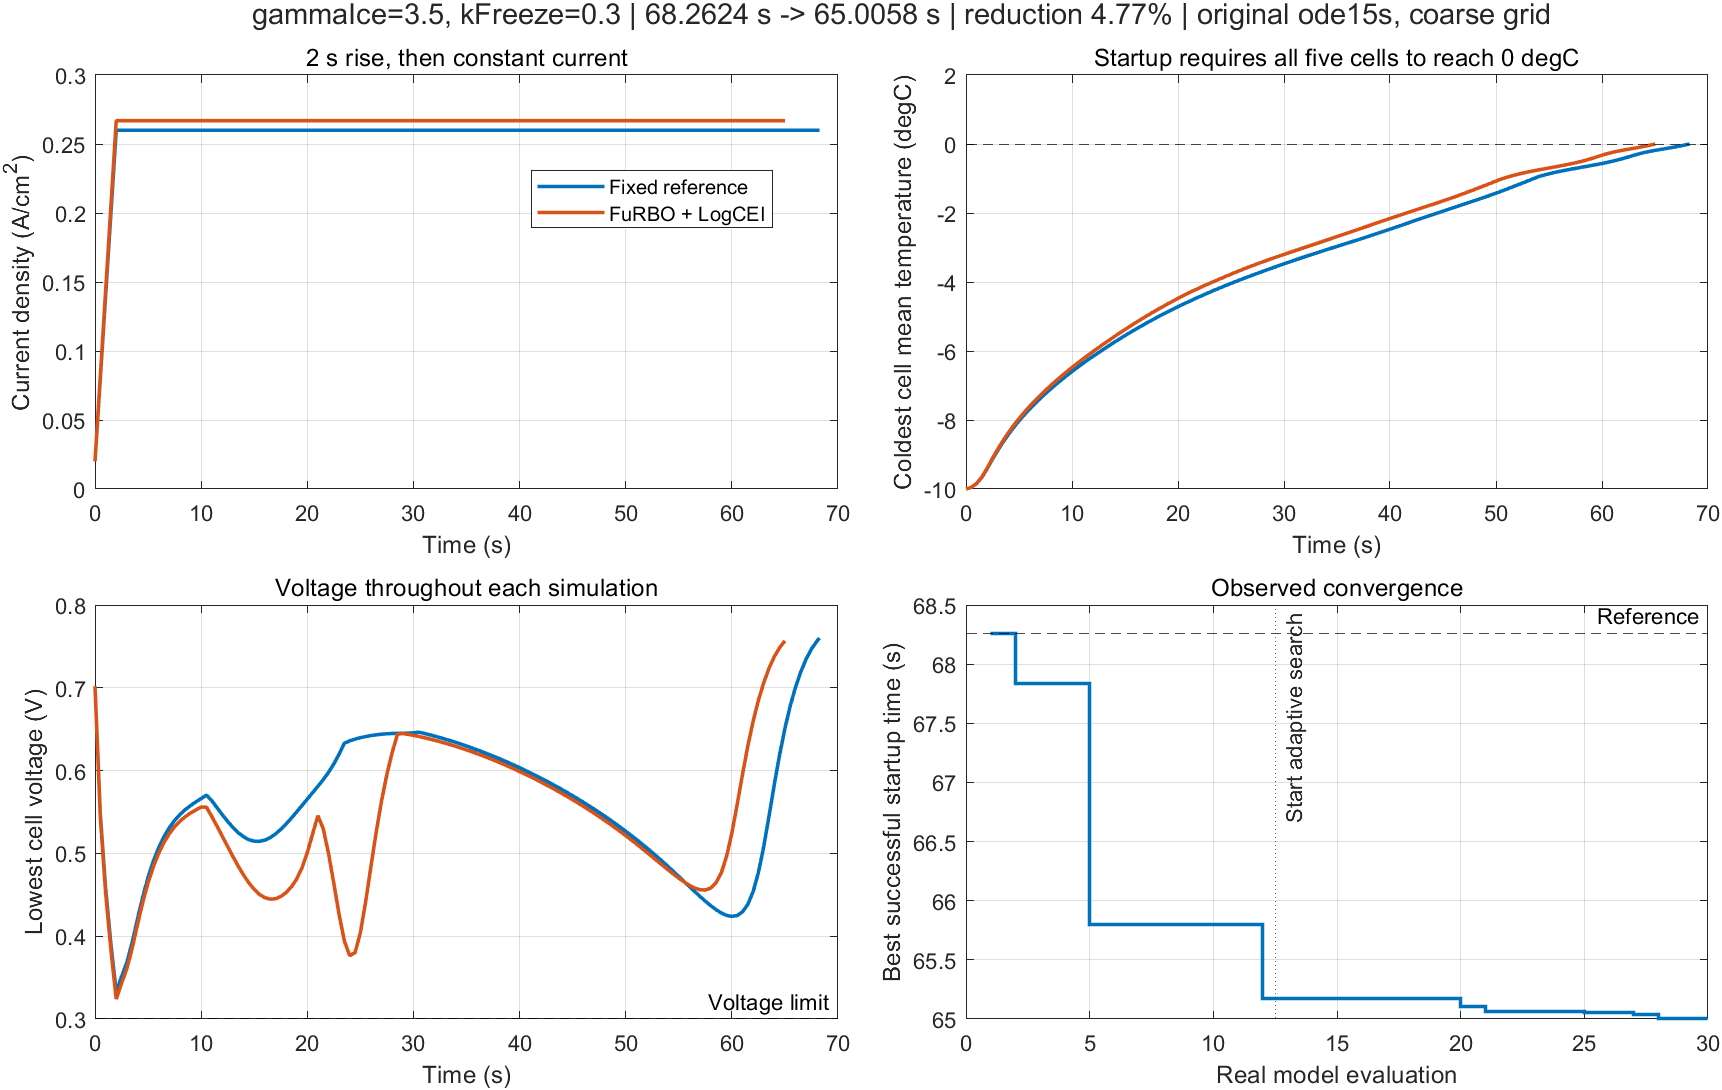
\includegraphics[width=0.98\linewidth]{figures/q2_constant_comparison_30eval.png}
  \caption{固定参考组与优化组的同网格对比：左上为加载电流密度曲线（$2~\mathrm{s}$ 升流后保持恒流），右上为最冷单片平均温度（虚线为 $0~^{\circ}\mathrm{C}$ 启动线），左下为全程最低单片电压（虚线为 $0.30~\mathrm{V}$ 下限），右下为历次真实评价中最佳成功启动时间的收敛过程（虚线为固定参考组，竖点线为初始采样结束、自适应选点开始）}
  \label{fig:q2-cc-comparison}
\end{figure}

与线性升载情形相比，恒流优化的改善幅度较小：优化组平台电流仅比参考组提高约 $2.67\%$，启动时间缩短 $4.77\%$。这符合恒流加载只有单自由度可调的事实，也说明 $-10~^{\circ}\mathrm{C}$ 初温下该协议的可优化裕度有限。约束分析显示电压下限仍是首要瓶颈：优化组全程最低单片电压 $0.324078~\mathrm{V}$，距 $0.30~\mathrm{V}$ 下限仅 $0.0241~\mathrm{V}$；启动时累积电荷 $17.1019~\mathrm{C\,cm^{-2}}$，仅为上限的 $85.5\%$；平台电流远未触及 $0.5~\mathrm{A\,cm^{-2}}$ 上限。继续提高平台电流首先会使单片电压提前触限，而非触及电荷或冰量上限，与线性升载情形的结论一致。表中结果为 30 次预算内的最佳实测值，不代表全局最优。

\subsubsection{最低自启动初温}
\label{subsec:q2-cc-mintemp}

将优化后的加载曲线固定，在粗网格模型下搜索最低可自冷启动初温：先在已验证的 $-10~^{\circ}\mathrm{C}$ 结果基础上以 $1~^{\circ}\mathrm{C}$ 步长向下试算 $-11$、$-12~^{\circ}\mathrm{C},\ldots$，直至首次失败；再在最近成功初温与最近失败初温之间二分细化，直至区间宽度小于 $0.01~^{\circ}\mathrm{C}$。每次试算同时将电堆初温与环境温度设为待测温度，加载曲线与模型参数保持不变，不在各初温下重新优化。

\begin{table}[H]
  \centering
  \caption{固定优化恒流曲线下的最低初温搜索结果}
  \label{tab:q2-cc-mintemp}
  \small
  \begin{tabularx}{0.94\linewidth}{>{\centering\arraybackslash}X>{\centering\arraybackslash}X>{\centering\arraybackslash}X>{\centering\arraybackslash}X>{\centering\arraybackslash}X>{\centering\arraybackslash}X}
    \toprule
    初温/$^{\circ}\mathrm{C}$ & 结果 & 启动/终止时间/s & 最低单片电压/V & 累计电荷/$(\mathrm{C\,cm^{-2}})$ & 最大局部冰体积分数\\
    \midrule
    $-10$ & 成功 & 65.005821 & 0.324078 & 17.101926 & —\\
    $-11$ & 成功 & 73.382959 & 0.316168 & 19.337628 & 0.398985\\
    $-11.0703125$ & 成功 & 73.916039 & 0.301405 & 19.479895 & 0.400590\\
    $-11.078125$ & 失败 & 64.737831 & 0.300000 & 17.030408 & 0.400203\\
    \bottomrule
  \end{tabularx}
\end{table}

在已测试的固定曲线与粗网格模型下，最冷的已验证成功初温为 $-11.0703125~^{\circ}\mathrm{C}$，紧邻的 $-11.078125~^{\circ}\mathrm{C}$ 失败；若临界点附近的成功性随初温单调变化，临界初温位于两者之间，区间宽度约 $0.0078~^{\circ}\mathrm{C}$。因此宜报告“约 $-11.07~^{\circ}\mathrm{C}$（数值搜索结果）”，不应把小数位当作物理测量精度。

失败工况的分析给出直接失效路径。在 $-11.078125~^{\circ}\mathrm{C}$ 下，第 1 片最先在 $64.7378~\mathrm{s}$ 降至 $0.30~\mathrm{V}$；此时第 1 片平均温度约 $-0.599~^{\circ}\mathrm{C}$、最大局部冰体积分数约 $0.4002$，第 5 片约 $-0.247~^{\circ}\mathrm{C}$，而第 2–4 片已高于 $2~^{\circ}\mathrm{C}$。冰体积分数与累计电荷均未达到各自上限，端部第 1 片持续偏冷、局部结冰及随之加重的电压损失构成直接失败路径。成功工况在约 $65~\mathrm{s}$ 处最低单片电压仍为 $0.301405~\mathrm{V}$，随后电压恢复并最终完成升温，说明 $-11.07~^{\circ}\mathrm{C}$ 附近的启动对电压裕度高度敏感。

该最低初温是固定加载曲线、粗网格下的数值搜索结果，尚未用完整网格验证，也不能据此声称允许重新优化加载曲线时的全局最低初温。

\subsection{线性升载策略}
\label{subsec:q2-linear}

线性升载策略以初始电流密度、升载速率与平台电流密度三个参数刻画电流曲线，是恒流加载的自然推广。下面依次给出其优化模型、求解方法、仿真设置与优化结果分析。

\subsubsection{优化模型}

线性加载曲线由初始电流密度 $j_0$、升载速率 $r$ 和平台电流密度 $j_p$ 决定：
\begin{equation}
  j(t;\bm{\theta})=\min\{j_0+rt,j_p\},
  \qquad \bm{\theta}=(j_0,r,j_p).
  \label{eq:q2-linear-current}
\end{equation}
搜索范围取
\begin{equation}
  0\le j_0\le0.50,\qquad
  0.001\le r\le0.050,\qquad
  j_0\le j_p\le0.50,
  \label{eq:q2-search-domain}
\end{equation}
为提高代理模型的数值稳定性，将三个变量归一化到 $[0,1]^3$：
\begin{equation}
  x_1=\frac{j_0}{0.50},\qquad
  x_2=\frac{r-0.001}{0.049},\qquad
  x_3=\frac{j_p-j_0}{0.50-j_0}.
\end{equation}

定义启动时刻 $t_s$ 为五片单电池平均温度全部首次达到 $0~^{\circ}\mathrm{C}$ 的时刻。优化问题为
\begin{align}
  \min_{\bm{\theta}}\quad & t_s(\bm{\theta}), \label{eq:q2-objective}\\
  \text{s.t.}\quad
  & \min_{1\le k\le5}\bar T_k(t_s)\ge273.15~\mathrm{K}, \nonumber\\
  & 0\le j(t)\le0.50~\mathrm{A\,cm^{-2}}, \quad 0\le t\le t_s, \nonumber\\
  & q_{\mathrm{use}}(t_s)\le20~\mathrm{C\,cm^{-2}}, \nonumber\\
  & \min_{1\le k\le5}V_k(t)\ge0.30~\mathrm{V}, \quad 0\le t\le t_s, \nonumber\\
  & \max_{k,x}\varepsilon_{\mathrm{ice},k}(x,t)<0.99, \quad 0\le t\le t_s, \nonumber\\
  & \max_{k,x}\left(\varepsilon_{l,k}+\varepsilon_{i,k}\right)<0.98,
  \quad 0\le t\le t_s. \nonumber
\end{align}
因此，线性加载优化的实质是在允许的 $j_0$、$r$ 和 $j_p$ 范围内，寻找使五片单电池全部升至 $0~^{\circ}\mathrm{C}$ 所需时间最短的加载曲线，同时保证启动全过程满足电流、电量、电压和冰水含量约束。数值仿真中，若任一约束在达到启动条件前被触发，则相应参数组合判定为不可行；否则记录其实际启动时间作为目标函数值。

\subsubsection{求解方法}
\label{subsec:q2-linear-method}

单次五片冷启动仿真包含刚性微分方程和事件终止，目标函数不光滑，且一次真实评估成本较高。本文采用受可行性驱动信赖域贝叶斯优化 FuRBO 启发的候选区域构造方法~\cite{ascia2025furbo}，并用 LogEI 代替 FuRBO 原算法的联合 Thompson 采样采集函数~\cite{ament2023logei}。因此，本方法是面向本题的组合式实现，并非 FuRBO 的严格复现。

对已评价样本分别建立两个高斯过程代理模型：可行性模型以启动成功或失败的二元标签为训练目标，时间模型只拟合成功样本的 $t_s$。每轮以当前最佳真实可行点为中心，在半径为 $R$ 的球内生成检查点；根据预测可行概率与预测启动时间选出较优检查点，并用其包络得到本轮超矩形信赖域。在该区域内先用拉丁超立方生成候选，再最大化
\begin{equation}
  \log a(\bm{x})=
  \operatorname{LogEI}\!\left(\bm{x};t_s^{\mathrm{best}}\right)
  +\log P\!\left(\mathrm{feasible}\mid\bm{x}\right).
  \label{eq:q2-acquisition}
\end{equation}
LogEI 与普通期望改进具有相同或近似相同的最优点，但能避免期望改进在小数值区域下溢，使候选排序更稳定。代理模型只用于选择下一次评价点；最终报告的最优解必须经过完整的五片物理模型重新计算。

\begin{algorithm}[H]
  \caption{可行性驱动信赖域贝叶斯搜索（以线性加载参数为例）}
  \label{alg:q2-search}
  \begin{algorithmic}[1]
    \REQUIRE 归一化搜索域 $[0,1]^3$，真实五片模型，最大评价次数
    \STATE 用最大最小准则拉丁超立方生成初始样本并逐一真实仿真
    \WHILE{真实模型评价次数未达到上限}
      \STATE 用有效样本拟合可行性高斯过程，用成功样本拟合启动时间高斯过程
      \STATE 以当前最佳真实可行点为中心，在半径 $R$ 内生成检查点
      \STATE 由较优检查点构造超矩形信赖域，并生成候选点集
      \STATE 按式\eqref{eq:q2-acquisition}排序，选择与历史样本不重复的候选点
      \STATE 调用真实五片模型，记录启动时间、约束状态与数值求解状态
      \STATE 连续两次改进则扩大信赖域；连续三次未改进则缩小信赖域
    \ENDWHILE
    \ENSURE 返回真实仿真中启动时间最短的可行方案
  \end{algorithmic}
\end{algorithm}

实现中使用 \texttt{fitrgp} 拟合自动相关长度平方指数核高斯过程，使用 \texttt{lhsdesign} 生成初始样本、检查区域内的候选点，并保存评价记录与信赖域状态以便断点续算。数值失败样本消耗评价预算，但不作为物理不可行标签训练可行性模型，从而避免把求解器故障误判为电堆失效。

\subsubsection{仿真设置}

未优化方案与优化方案均在相同物理参数、相同快速网格和相同求解容差下重新计算，设置见\Cref{tab:q2-settings}。该公平对比避免了历史检查点、网格和容差不同造成的偏差。

\begin{table}[H]
  \centering
  \caption{问题二线性加载对比的主要仿真设置}
  \label{tab:q2-settings}
  \begin{tabularx}{0.94\linewidth}{>{\raggedright\arraybackslash}X>{\centering\arraybackslash}p{0.31\linewidth}>{\raggedright\arraybackslash}p{0.31\linewidth}}
    \toprule
    设置项 & 取值 & 说明\\
    \midrule
    初始温度 & $-10~^{\circ}\mathrm{C}$ & 五片单电池与两块端板同温初始化\\
    单片快速网格 & $[2,3,4,4,2]$ & 依次对应五个功能层\\
    相变与冰覆盖参数 & $k_{\mathrm{freeze}}=0.4~\mathrm{s^{-1}}$，$\gamma_{\mathrm{ice}}=3.5$ & 本结果包的快速计算口径\\
    相变平滑宽度 & $0.2~\mathrm{K}$ & 消除冰点附近硬切换导致的步长失败\\
    求解器容差 & $\mathrm{RelTol}=5\times10^{-5}$，$\mathrm{AbsTol}=5\times10^{-9}$ & 两个方案完全一致\\
    最大步长与输出步长 & $0.05~\mathrm{s}$，$0.5~\mathrm{s}$ & 启动事件由求解器连续定位\\
    端板与双极板处理 & 独立端板，共享双极板计数 & 避免端板同温假设和双极板热容重复计数\\
    约束阈值 & $j\le0.50$，$V_k\ge0.30$，$q_{\mathrm{use}}\le20$ & 全过程事件约束\\
    冰与孔隙阈值 & $\varepsilon_{\mathrm{ice}}<0.99$，$\varepsilon_l+\varepsilon_i<0.98$ & 对全部单片与空间节点检查\\
    \bottomrule
  \end{tabularx}
\end{table}

本节参数用于复现当前结果包；最终验证时应与问题一的标定口径统一，并以完整网格复核。

\subsubsection{优化结果与约束分析}

未优化线性方案取 $j_0=0.0200~\mathrm{A\,cm^{-2}}$、$r=0.0100~\mathrm{A\,(cm^2\,s)^{-1}}$、$j_p=0.4000~\mathrm{A\,cm^{-2}}$。真实模型搜索得到的优化方案为
\begin{equation}
  j_0=0.117641245~\mathrm{A\,cm^{-2}},\qquad
  r=0.008079398~\mathrm{A\,(cm^2\,s)^{-1}},\qquad
  j_p=0.447158213~\mathrm{A\,cm^{-2}}.
  \label{eq:q2-best-strategy}
\end{equation}
同网格复算结果见\Cref{tab:q2-results}与\Cref{fig:q2-linear-comparison}。

\begin{table}[H]
  \centering
  \caption{未优化与优化线性加载方案的同网格仿真结果}
  \label{tab:q2-results}
  \begin{tabular}{lcc}
    \toprule
    指标 & 未优化方案 & 优化方案\\
    \midrule
    $j_0/(\mathrm{A\,cm^{-2}})$ & 0.020000 & 0.117641\\
    $r/(\mathrm{A\,(cm^2\,s)^{-1}})$ & 0.010000 & 0.008079\\
    $j_p/(\mathrm{A\,cm^{-2}})$ & 0.400000 & 0.447158\\
    启动时间 $t_s/\mathrm{s}$ & 48.838845 & 40.726546\\
    启动时累积电荷 $q_{\mathrm{use}}/(\mathrm{C\,cm^{-2}})$ & 12.315537 & 11.491596\\
    全程最低单片电压 $V_{\min}/\mathrm{V}$ & 0.406337 & 0.311870\\
    全程最大局部冰体积分数 & 0.343339 & 0.331563\\
    启动时最大局部冰体积分数 & 0.189204 & 0.197514\\
    启动时电流密度 $j(t_s)/(\mathrm{A\,cm^{-2}})$ & 0.400000 & 0.446687\\
    \bottomrule
  \end{tabular}
\end{table}

优化方案使启动时间缩短 $8.1123$ s，相对降幅为 $16.61\%$；累积电荷减少 $0.8239$ C/cm$^2$，下降 $6.69\%$。启动提前并非通过无条件提高平台电流实现。优化器把初始电流从 $0.0200$ A/cm$^2$ 提高到 $0.1176$ A/cm$^2$，使冷启动早期更快地产生反应热；随后采用略低的升载斜率，使电流增长与膜水合、温升和融冰过程相匹配，从而在电压不越界的前提下持续增加产热。

\Cref{fig:q2-linear-comparison}左上图显示，未优化方案在 $38.0~\mathrm{s}$ 达到 $0.4000~\mathrm{A\,cm^{-2}}$ 的平台，之后继续恒流加热约 $10.84~\mathrm{s}$ 才启动。优化方案的理论平台到达时间为
\begin{equation}
  t_p=\frac{j_p-j_0}{r}=40.7848~\mathrm{s},
\end{equation}
而模型在 $40.7265~\mathrm{s}$ 已启动，此时 $j=0.446687~\mathrm{A\,cm^{-2}}$。因此，优化曲线在启动前尚未真正进入平台阶段，不能将图中的末段表述为已形成稳定平台。

温度结果表明，优化后最冷单片更早达到 $0~^{\circ}\mathrm{C}$。启动时五片平均温度依次约为 $0$、$5.061$、$6.608$、$5.238$ 和 $0.365~^{\circ}\mathrm{C}$，中部单片温升更快，第一片仍是决定启动时刻的热约束单片。此时左右端板温度约为 $-6.32$ 和 $-6.28~^{\circ}\mathrm{C}$，说明将端板设为独立热节点是必要的；若强制端板与端部单片同温，将明显改变端部热惯性与启动判定。

电压约束是继续缩短启动时间的主要瓶颈。优化方案的全程最低单片电压为 $0.311870$ V，出现在约 $36$ s 的第4片，距离 $0.30$ V 下限仅 $0.011870$ V。此后尽管电流仍在上升，温升、膜水合改善及局部融冰使电压重新回升。相比之下，电流上限尚有约 $0.0533$ A/cm$^2$ 的余量，累积电荷只使用上限的 $57.46\%$，冰体积分数和孔隙占用也远未达到失败阈值。因此，在当前模型参数下，简单提高初始电流或升载速率首先会触及单片低电压边界，而不是电荷或冰量上限。

冰量曲线显示，优化方案的最大局部冰体积分数在约 $39~\mathrm{s}$ 达到 $0.3316$，随后随局部温度接近冰点而快速下降，启动时降至 $0.1975$。全程最大冰量出现在第1片，与其端部散热较强、温升最慢相一致；最低电压却出现在第4片，说明热约束、冰约束和电压约束不一定由同一片电池控制。加载策略必须对五片电池的完整历史同时检查，不能只依据平均堆温或总电压判断启动是否安全。

\begin{figure}[H]
  \centering
  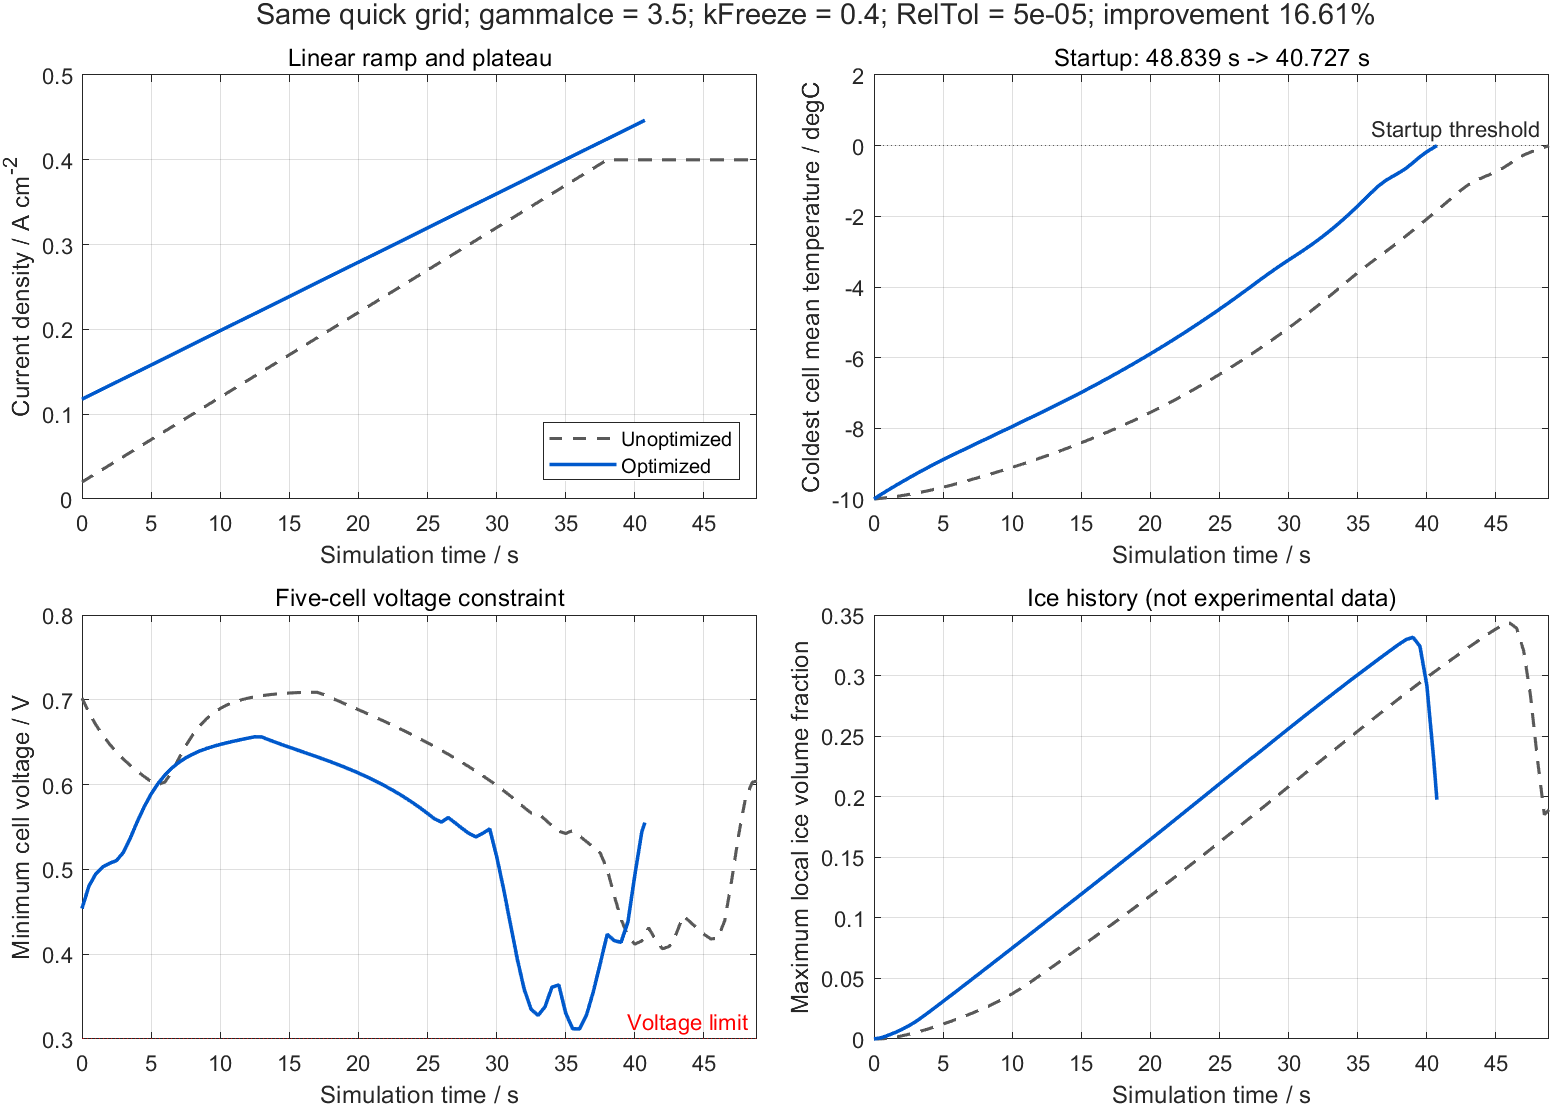
\includegraphics[width=0.98\linewidth]{figures/q2_linear_comparison.png}
  \caption{未优化与优化线性加载方案在同一快速网格下的模型仿真对比}
  \label{fig:q2-linear-comparison}
\end{figure}

将求解器相对容差和绝对容差在对比设置基础上再收紧一倍，优化方案仍成功启动，得到 $40.7242~\mathrm{s}$，与表中结果仅相差约 $0.0023~\mathrm{s}$。这说明该候选点对当前快速网格上的时间积分容差不敏感，但尚不能替代空间完整网格验证。

% ===== 分段阶梯加载策略（五档九变量结果包） =====

\subsection{分段阶梯加载策略}
\label{subsec:q2-step}

分段阶梯加载以若干恒流档位近似任意电流曲线：档位越多，对连续曲线的逼近能力越强，但待定参数也越多。本节先给出四档未优化基准，再对五档曲线的全部九个参数（五个档位电流与四个切换时刻）进行联合优化。

\subsubsection{优化模型}
\label{subsec:q2-step-model}

五档阶梯加载曲线由五个档位电流与四个切换时刻完全确定：
\begin{equation}
  j(t;\bm{\theta})=j_i,\quad t_{i-1}\le t<t_i,\ i=1,\ldots,5,
  \qquad
  \bm{\theta}=(j_1,\ldots,j_5,t_1,\ldots,t_4),
  \label{eq:q2-step-current}
\end{equation}
其中 $t_0=0$，并约定 $t\ge t_4$ 后保持 $j_5$。五个档位电流的物理范围均为 $[0,0.5]~\mathrm{A\,cm^{-2}}$；四个切换时刻依次在互不重叠的数值搜索窗 $[1,8]$、$[8.1,16.9]$、$[17,23.9]$、$[24,38]~\mathrm{s}$ 内搜索。归一化方式为
\begin{equation}
  x_i=\frac{j_i}{0.5}\ (i=1,\ldots,5),\qquad
  x_{5+k}=\frac{t_k-t_k^{\mathrm{L}}}{t_k^{\mathrm{U}}-t_k^{\mathrm{L}}}\ (k=1,\ldots,4),
  \label{eq:q2-step-decode}
\end{equation}
其中 $t_k^{\mathrm{L}}$、$t_k^{\mathrm{U}}$ 为第 $k$ 个切换时刻搜索窗的上下界。需要强调的是，切换时刻的搜索窗只是数值搜索范围而非题目给定的物理界限，若最优点落在某窗口边界，应扩窗复核。目标函数与约束与式\eqref{eq:q2-objective}相同，此时优化问题为九维变量空间上的启动时间最小化。

未优化基准采用可启动的四档曲线 $(j_1,j_2,j_3,j_4)=(0.15,0.18,0.30,0.40)~\mathrm{A\,cm^{-2}}$、切换时刻 $(5,15,35)~\mathrm{s}$。其档位与切换时刻均未经优化，只用于衡量阶梯加载在未经参数选择时的启动性能。

\subsubsection{求解方法}
\label{subsec:q2-step-method}

求解沿用与前两节相同的可行性驱动信赖域贝叶斯优化框架（算法~\ref{alg:q2-search} 与式\eqref{eq:q2-acquisition}），针对九维空间做如下配置。信赖域初始半径 $R_0=0.65$、下限 $0.10$，连续两次改进加倍、连续三次未改进减半；每轮生成 $512$ 个球内检查点，由预测最优的前 $10\%$ 构造超矩形信赖域，并强制把当前最优真实可行点纳入检查点集合，避免代理排序失真时信赖域偏离该任职点。候选池含 $512$ 个信赖域内拉丁超立方样本，并混入 $20\%$ 的全局候选，另每 $6$ 轮强制一次全局探查，以缓解九维信赖域的局部化风险；候选点与已有成功点的归一化距离超过 $0.32$ 时被剔除。采集函数为解析 LogEI 与对数可行概率之和，并在可行概率上叠加经验邻域校正项（带宽 $0.6R$、权重 $0.5$），抑制稀疏样本下高斯过程的过度自信；当池内最高可行概率低于 $0.10$ 时转入纯可行性营救模式。采集函数本身在信赖域内以对数变换配合 Nelder–Mead 局部精修，取 $3$ 个不同初值。

约束学习采用事件感知方式：事件驱动的求解器恰好终止在约束边界上，失败样本的电压裕度常为零，仅学习二元成功标签会低估较早失败的严重性；因此在符号化违例指标 $G$ 上叠加早期事件惩罚项 $0.01+0.25\max(0,(60-t_{\mathrm{term}})/60)$，其中 $t_{\mathrm{term}}$ 为终止时刻。数值失败样本与“在已知最快启动时间加 $0.5~\mathrm{s}$ 的截止前未启动”的时间截断样本均不参与代理模型训练；时间截断用于控制单次评价成本，不计为物理失败。历史真实仿真仅在物理源码与设置完全一致的校验戳下复用，换路径后的首次运行会重新仿真已发表最优点。

该实现是 FuRBO 与 LogEI 的工程化组合（全局候选混合、事件感知约束学习、经验邻域校正、任职点锚定与时间截断），并非两篇文献算法的逐字复现。

\subsubsection{仿真设置}
\label{subsec:q2-step-settings}

本结果包与线性升载结果包采用相同的快速计算口径：$k_{\mathrm{freeze}}=0.4~\mathrm{s^{-1}}$（取题目给定范围 $0.3\sim0.5~\mathrm{s^{-1}}$ 的中点）、$\gamma_{\mathrm{ice}}=3.5$、粗网格 $[2,3,4,4,2]$、$\mathrm{RelTol}=10^{-4}$、$\mathrm{AbsTol}=10^{-8}$、孔隙占用阈值 $0.98$，其余设置与\Cref{tab:q2-settings}一致。最优方案另行用更严格容差（$\mathrm{RelTol}=5\times10^{-5}$、$\mathrm{AbsTol}=5\times10^{-9}$）独立复核。

\subsubsection{优化结果与约束分析}
\label{subsec:q2-step-results}

同网格复算结果见\Cref{tab:q2-step-results}与\Cref{fig:q2-step-comparison}。

\begin{table}[H]
  \centering
  \caption{未优化四档与优化五档阶梯加载的仿真结果}
  \label{tab:q2-step-results}
  \small
  \begin{tabularx}{0.94\linewidth}{>{\raggedright\arraybackslash}X>{\raggedright\arraybackslash}p{0.30\linewidth}>{\raggedright\arraybackslash}p{0.30\linewidth}}
    \toprule
    指标 & 未优化四档 & 优化五档\\
    \midrule
    档位电流/$(\mathrm{A\,cm^{-2}})$ & 0.15, 0.18, 0.30, 0.40 & 0.1752, 0.2914, 0.2427, 0.2618, 0.4598\\
    切换时刻/s & 5, 15, 35 & 2.5713, 12.1507, 20.5979, 27.5905\\
    启动时间 $t_s/\mathrm{s}$ & 45.8918 & 36.0266（严格容差复核 36.0275）\\
    全程最低单片电压 $V_{\min}/\mathrm{V}$ & 0.387167 & 0.314724（严格复核值）\\
    启动时累积电荷 $q_{\mathrm{use}}/(\mathrm{C\,cm^{-2}})$ & 12.906723 & 11.002117（严格复核值）\\
    启动时最大局部冰体积分数 & 0.198985 & 0.192016（严格复核值）\\
    \bottomrule
  \end{tabularx}
\end{table}

优化使启动时间缩短 $9.8652~\mathrm{s}$，相对降幅 $21.50\%$。这一改善同时包含曲线结构（四档变为五档）与参数两方面的变化，不能全部归因于优化算法：同属五档曲线时，原先固定前缀的九变量方案为 $36.5010~\mathrm{s}$，全部九参数联合优化进一步缩短至 $36.0266~\mathrm{s}$，即算法带来的净改善为 $0.4744~\mathrm{s}$（$1.30\%$）。严格容差复核得到 $36.0275~\mathrm{s}$，与快网格结果仅相差 $0.0009~\mathrm{s}$，表明最优候选对时间积分容差不敏感。

\begin{figure}[H]
  \centering
  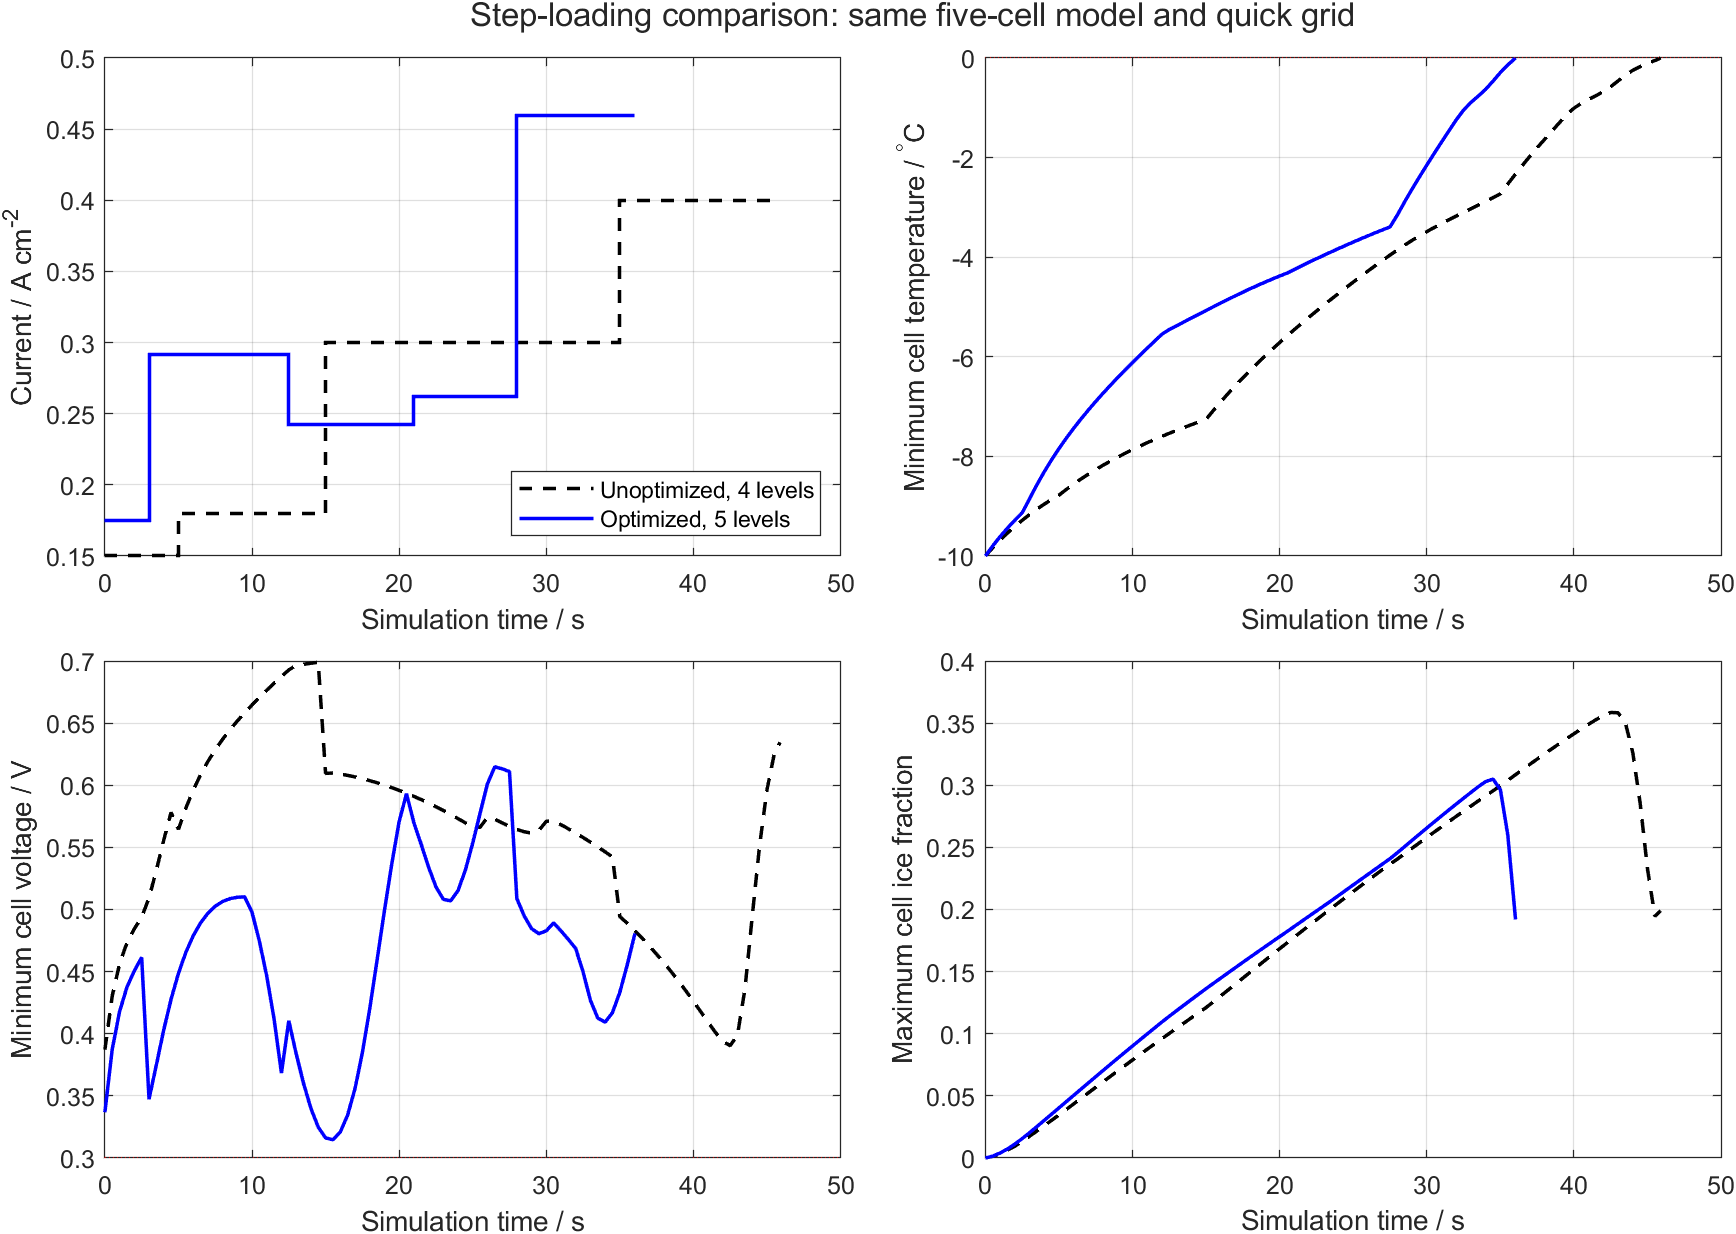
\includegraphics[width=0.98\linewidth]{figures/q2_step_loading_comparison.png}
  \caption{未优化四档与优化五档阶梯加载的同网格对比：左上为电流阶梯曲线，右上为最冷单片平均温度（红虚线为 $0~^{\circ}\mathrm{C}$ 启动线），左下为全程最低单片电压（红虚线为 $0.30~\mathrm{V}$ 下限），右下为最大局部冰体积分数}
  \label{fig:q2-step-comparison}
\end{figure}

优化五档的结构值得分析：首档 $0.1752~\mathrm{A\,cm^{-2}}$ 与四档基准的首档相当，避免低水合阶段的电压骤降；第二档显著提高到 $0.2914~\mathrm{A\,cm^{-2}}$，在膜开始升温后尽快加大产热；第三、四档回落到 $0.2427$ 与 $0.2618~\mathrm{A\,cm^{-2}}$，避让电压低点；末档 $0.4598~\mathrm{A\,cm^{-2}}$ 已接近 $0.5~\mathrm{A\,cm^{-2}}$ 上限，在电压裕度恢复后全力加热。四个切换时刻均落在搜索窗内部，未触碰窗口边界。严格复核的全程最低单片电压 $0.314724~\mathrm{V}$，距 $0.30~\mathrm{V}$ 下限仅 $0.0147~\mathrm{V}$；启动时累积电荷 $11.0021~\mathrm{C\,cm^{-2}}$，仅为上限的 $55.0\%$；启动时最大局部冰体积分数 $0.1920$，远未达到冰量阈值。末档电流未进一步增大，是因为继续提高末档电流会提前触及单片低电压边界而非电荷或冰量上限——电压约束再次成为限制启动速度的首要瓶颈，与恒流、线性升载两节的结论一致。

该结果为当前模型、参数与快速网格下搜索预算内的最佳实测值，不声称全局最优；启动时间尚未实现 $30~\mathrm{s}$ 以内，完整网格与实验数据的最终验证仍有待完成。

\subsubsection{最低自启动初温}
\label{subsec:q2-step-mintemp}

固定优化五档曲线，以二分方式搜索最低可自冷启动初温，每次试算同时将电堆初温与环境温度设为待测温度。快速网格容差下，已验证的最冷成功初温为 $-10.59375~^{\circ}\mathrm{C}$，相邻的 $-10.625~^{\circ}\mathrm{C}$ 失败，边界区间宽 $0.03125~^{\circ}\mathrm{C}$；用更严格容差复核后，最冷成功初温为 $-10.609375~^{\circ}\mathrm{C}$（启动时间 $37.5900~\mathrm{s}$），相邻失败点仍为 $-10.625~^{\circ}\mathrm{C}$，区间宽 $0.015625~^{\circ}\mathrm{C}$。因此宜报告优化阶梯曲线的最低自启动初温约为 $-10.61~^{\circ}\mathrm{C}$（严格容差下的数值搜索结果）。

严格容差下，成功工况 $-10.609375~^{\circ}\mathrm{C}$ 的全程最低单片电压为 $0.300289~\mathrm{V}$，仅比 $0.30~\mathrm{V}$ 下限高 $2.9\times10^{-4}~\mathrm{V}$，说明该曲线在临界初温附近的启动完全受电压下限支配。失败工况 $-10.625~^{\circ}\mathrm{C}$ 由第 $1$ 片在 $34.7749~\mathrm{s}$ 触发 $0.30~\mathrm{V}$ 电压事件，此时最冷单片（第 $1$ 片）平均温度约 $-0.883~^{\circ}\mathrm{C}$，全程最大局部冰体积分数 $0.3103$、累计电荷 $10.426~\mathrm{C\,cm^{-2}}$，均未达到各自上限——端部单片的低电压仍是直接失效路径，与恒流曲线下的初温搜索结论一致。

需要说明，本节最低初温采用 $k_{\mathrm{freeze}}=0.4~\mathrm{s^{-1}}$ 的结果包口径，而恒流曲线的最低初温（约 $-11.07~^{\circ}\mathrm{C}$）来自 $k_{\mathrm{freeze}}=0.3~\mathrm{s^{-1}}$ 的结果包，两者不宜直接比较；加载策略对最低初温的影响应在统一口径下另行评估。该初温亦未在完整网格上验证，不排除重新优化曲线后获得更低初温的可能。
% ===== 待补：三种加载策略的统一比较（恒流与阶梯曲线的最低初温已分别分析，但 kFreeze 口径不同，统一口径下的比较待补） =====

\section{问题三模型的建立与求解}
\label{sec:model3}

\subsection{模型建立}
在电堆能量守恒方程中引入各片独立的辅助加热源项，建立 $-30~^{\circ}\mathrm{C}$ 下的电堆辅助冷启动模型，并分别给出纯预加热启动与恒定功率协同启动两种方式下以辅助加热总能耗为目标的优化问题。

\subsection{模型求解与结果}
求解两种方式下的最优加热功率分配与加热持续时间，给出总启动时间、各片能耗分配与总能耗，并比较二者在能耗、启动速度与端部单电池冰堵抑制效果上的差异。

\section{问题四模型的建立与求解}
\label{sec:model4}

\subsection{模型建立}
允许各片加热功率随时间独立调节，以实时测得的单片温度与电压为反馈信号建立动态功率控制模型，并施加功率限幅、冰体积分数阈值与电压安全下限等约束。

\subsection{模型求解与结果}
针对完全冷却与冷却 20~min、40~min 三种初始状态求解动态控制策略，并与恒功率策略在能耗、启动时间、最大温差等指标上比较；进一步给出冷却时间在 10--100~min 内变化时的温度场及恒功率策略下的冷启动结果。

\section{模型检验与灵敏度分析}
\label{sec:validation}

\subsection{模型检验}
将模型输出与已知结果、保留数据或基准方法进行比较，检查结果是否满足实际约束。若采用误差指标，应写清定义、计算范围和比较方式，避免仅凭图形相似就认定模型有效。

以观测值 $y_i$ 和预测值 $\hat y_i$ 为例，均方根误差可写为
\begin{equation}
  \operatorname{RMSE}
  =\sqrt{\frac{1}{N_s}\sum_{i=1}^{N_s}(y_i-\hat y_i)^2}.
\end{equation}
误差分析应结合问题的量纲与实际需求解释，必要时分别讨论总体误差和局部误差。

\subsection{灵敏度分析}
选择对结论可能有显著影响的参数，在合理区间内逐一改变或联合扰动，观察目标函数、决策变量及约束满足情况的变化。

\subsubsection{参数扰动方案}
说明扰动范围、采样方式以及其他参数是否保持不变。若参数由数据估计得到，扰动幅度应尽量与估计误差或实际变化范围相一致。

\subsubsection{稳健性讨论}
结合扰动结果讨论模型结论是否稳定，指出敏感参数以及需要提高测量精度的环节。出现不稳定现象时，应分析其来自数据、模型结构还是求解算法。

\section{模型评价与推广}

\subsection{模型的优点}
结合建模过程与检验结果说明模型的优势，例如变量含义清晰、约束表达完整、求解效率适用或结论具有可解释性。每项优点都应有相应依据。

\subsection{模型的局限}
说明假设简化、数据质量、参数估计以及算法近似带来的限制。局限应对应实际存在的问题，并尽量给出其可能影响结论的方向。

\subsection{模型的推广}
说明模型可迁移到哪些相近问题、迁移时需要调整哪些条件，以及哪些结论不能直接推广。推广部分应与已有模型保持联系，避免脱离已完成的分析。

% ref.bib 中的条目按正文首次引用的顺序输出
\bibliographystyle{settings/gmcm}
\bibliography{ref}

% \appendix 自动生成带中文编号的“附录”一级标题；其下继续使用 \subsection。
\appendix

\subsection{补充材料}
\label{app:p1-details}

本节汇总问题一模型中用于数值求解的闭合关系、三态水分配关系及完整初边界条件。正文仅保留守恒方程、低温相变机理和电压修正的关键表达式。

\subsubsection{气体与水输运闭合关系}

气体有效扩散系数采用 Bruggeman 孔隙率修正：
\begin{equation}
  D_{k,\mathrm{eff}}=D_{k,\mathrm{ref}}\left(\frac{T}{298.15}\right)^{1.75}\varepsilon_g^{1.5}.
  \label{eq:dkeff}
\end{equation}
由于 $\varepsilon_g$ 随冰与液态水的积累而变化，对第 $i$ 个网格单元积分后显式保留孔隙率变化项：
\begin{equation}
  \frac{\mathrm{d}c_k}{\mathrm{d}t}
  =\frac{1}{\varepsilon_g}\left(-\frac{N_{k,f+1}-N_{k,f}}{\Delta x}+S_k-c_k\frac{\mathrm{d}\varepsilon_g}{\mathrm{d}t}\right).
  \label{eq:gasdisc}
\end{equation}

多孔介质中只有气态水参与扩散，膜内水以吸附态迁移，因此
\begin{equation}
  N_{\mathrm{vap}}=
  \begin{cases}
    -D_{w,\mathrm{eff}}\dfrac{\partial m_v}{\partial x}, & x\in\Omega_{\mathrm{aGDL}}\cup\Omega_{\mathrm{aCL}}\cup\Omega_{\mathrm{cCL}}\cup\Omega_{\mathrm{cGDL}},\\[2ex]
    -D_{w,\mathrm{mem}}\dfrac{\partial m_w}{\partial x}, & x\in\Omega_{\mathrm{pem}},
  \end{cases}
  \label{eq:nvap}
\end{equation}
其中 $D_{w,\mathrm{eff}}=D_{w,\mathrm{ref}}(T/298.15)^{1.75}\varepsilon_g^{1.5}$，$D_{w,\mathrm{mem}}$ 采用备注1 给出的含水量与温度关联式。CL|PEM 界面采用有限速率导通关系
\begin{equation}
  N_{w,\mathrm{CL|PEM}}
  =\zeta\,\frac{D_{w,\mathrm{mem}}\lambda_{\max}\rho_{\mathrm{pem}}M_w}{\mathrm{EW}\,L_{\mathrm{pem}}}
    \bigl(a_{\mathrm{CL}}-a_{\mathrm{pem}}\bigr),
  \label{eq:interface}
\end{equation}
式中 $a_{\mathrm{CL}}$ 与 $a_{\mathrm{pem}}$ 为界面两侧水活度，$\zeta=30$，$\lambda_{\max}=22$。

液态水按 Darcy 定律在毛细压力梯度下排出：
\begin{equation}
  N_{\mathrm{liq}}=-\frac{\rho_l K_{\mathrm{eff}}k_{rl}}{\mu_l}\frac{\partial p_c}{\partial x},
  \label{eq:nliq}
\end{equation}
\begin{equation}
  p_c=-\sigma\cos\theta_c\sqrt{\frac{\varepsilon_0}{K_0}}\,J(s_l),
  \qquad
  J(s_l)=1.417s_l-2.12s_l^2+1.263s_l^3,
  \label{eq:pc}
\end{equation}
\begin{equation}
  K_{\mathrm{eff}}=K_0\left(\frac{\varepsilon_0-\varepsilon_i}{\varepsilon_0}\right)^{3},
  \qquad
  k_{rl}=s_l^{3},
  \qquad
  \mu_l=2.414\times10^{-5}\,10^{\frac{247.8}{T-140}}.
  \label{eq:kr}
\end{equation}
其中 $K_0$ 与 $\theta_c$ 取附件1 中 GDL 与 CL 的相应数值。电渗拖曳通量及拖曳系数为
\begin{equation}
  N_{\mathrm{eod}}=\frac{n_d M_w i_m}{F},
  \qquad
  n_d=2.5\frac{\lambda}{22}.
  \label{eq:neod}
\end{equation}
质子电流密度在 aCL 内由 $0$ 线性增至 $j$，在膜内恒为 $j$，在 cCL 内由 $j$ 线性降至 $0$。

\subsubsection{三态水分配与冰量约束}

阴极催化层离聚物结合水及孔隙水分别为
\begin{equation}
  m_{\mathrm{ion}}=\frac{\varepsilon_{\mathrm{ion}}\rho_{\mathrm{ion}}M_w}{\mathrm{EW}}\lambda_{\mathrm{cCL}},
  \qquad
  m_{\mathrm{pore}}=m_w-m_{\mathrm{ion}},
  \label{eq:mion}
\end{equation}
其中 $\varepsilon_{\mathrm{ion}}=0.3$。结合水不占据孔隙且不冻结。冰占据的体积分数与扣除冰后的孔隙率为
\begin{equation}
  \varepsilon_i=\frac{m_i}{\rho_{\mathrm{ice}}},
  \qquad
  s_i=\frac{\varepsilon_i}{\varepsilon_0},
  \qquad
  \varepsilon_{\mathrm{after}}=\varepsilon_0-\varepsilon_i.
  \label{eq:epsi}
\end{equation}
扣除冰后，可动水 $m_{\mathrm{mobile}}=m_{\mathrm{pore}}-m_i$ 按局部瞬时平衡分配：
\begin{equation}
  m_v=\min\!\left[m_{\mathrm{mobile}},~A(T)\,\varepsilon_{\mathrm{after}}\right],
  \qquad
  m_l=m_{\mathrm{mobile}}-m_v,
  \label{eq:vl}
\end{equation}
其中 $A(T)=M_w p_{\mathrm{sat}}(T)/(RT)$。孔隙达到气液饱和时，有
\begin{equation}
  m_l=\frac{m_{\mathrm{mobile}}-A(T)\,\varepsilon_{\mathrm{after}}}{1-A(T)/\rho_l},
  \qquad
  m_v=m_{\mathrm{mobile}}-m_l,
  \label{eq:mlsat}
\end{equation}
因此剩余气相孔隙率为
\begin{equation}
  \varepsilon_g=\varepsilon_{\mathrm{after}}-\frac{m_l}{\rho_l}
  =\varepsilon_0-\varepsilon_i-\frac{m_l}{\rho_l}.
  \label{eq:epsg}
\end{equation}
数值求解时还需限制
\begin{equation}
  0\le m_i\le \min\!\left(m_{\mathrm{pore}},~\rho_{\mathrm{ice}}\varepsilon_0\right),
  \label{eq:icelimit}
\end{equation}
即冰量不得超过现有孔隙水总量或干孔隙的容积上限。

\subsubsection{水合、热物性与电化学闭合关系}

水合方程（\ref{eq:hyd}）中的可供水量与反应产水速率为
\begin{equation}
  \lambda_{\mathrm{avail}}
  =\frac{m_{\mathrm{pore,cCL}}}{\varepsilon_{\mathrm{ion}}\rho_{\mathrm{ion}}M_w/\mathrm{EW}},
  \qquad
  \dot m_{w,\mathrm{rxn}}=\frac{M_wj}{2FL_{\mathrm{cCL}}}.
  \label{eq:hydclosure}
\end{equation}
低温下离聚物的最大非冻结含水量为
\begin{equation}
  \lambda_{\mathrm{sat}}(T)=
  \begin{cases}
    4.837, & T<223.15~\mathrm{K},\\[0.5ex]
    \left(-1.304+0.01479T-3.594\times10^{-5}T^2\right)^{-1}, & 223.15\le T<273.15~\mathrm{K},\\[0.5ex]
    22, & T\ge273.15~\mathrm{K}.
  \end{cases}
  \label{eq:lambdasat}
\end{equation}
等效体积热容与导热系数分别采用体积分数加权和串联热阻计算：
\begin{equation}
  (\rho c_p)_{\mathrm{eff}}
  =\frac{\sum_i\rho_i c_{p,i}\delta_i+2\rho_{\mathrm{bp}}c_{p,\mathrm{bp}}\delta_{\mathrm{bp}}}{L},
  \qquad
  k_{\mathrm{eff}}=\frac{L}{\sum_i\delta_i/k_i}.
  \label{eq:thermalprop}
\end{equation}
膜与催化层离聚物的质子电导率为
\begin{equation}
  \begin{aligned}
    \kappa_{\mathrm{pem}}
    &=(0.5139\lambda-0.326)\exp\!\left[1268\!\left(\frac{1}{303.15}-\frac{1}{T}\right)\right],\\
    \kappa_{\mathrm{CL}}
    &=\varepsilon_{\mathrm{ion}}^{1.5}(0.5139\lambda_{\mathrm{CL}}-0.326)
      \exp\!\left[1268\!\left(\frac{1}{303.15}-\frac{1}{T}\right)\right].
  \end{aligned}
  \label{eq:kappa}
\end{equation}
浓差极化所需的极限电流密度按串联扩散阻力计算：
\begin{equation}
  j_{\mathrm{lim}}=\frac{4F\,c_{\mathrm{O_2,cCL}}}{\displaystyle\sum_{i\,\in\,\mathrm{cCL}\cup\mathrm{cGDL}}\frac{\Delta x_i}{D_{\mathrm{O_2,eff},i}}}
  =\frac{4F\,D_{\mathrm{O_2,eq}}\,c_{\mathrm{O_2,cCL}}}{L_{\mathrm{diff}}},
  \qquad
  L_{\mathrm{diff}}=L_{\mathrm{cCL}}+L_{\mathrm{cGDL}}.
  \label{eq:jlim}
\end{equation}

\subsubsection{完整初始条件与边界条件}

模型的初始条件为
\begin{equation}
  \begin{aligned}
    &T(x,0)=T_0,\qquad
    m_i(x,0)=0,\qquad
    \lambda_{\mathrm{cCL}}(0)=\lambda_{\mathrm{cCL},0},\\
    &c_{\mathrm{H_2}}(x,0)=\frac{p_0}{RT_0},\quad x\in\Omega_{\mathrm{aGDL}}\cup\Omega_{\mathrm{aCL}};\qquad
    c_{\mathrm{O_2}}(x,0)=\frac{y_{\mathrm{O_2}}p_0}{RT_0},\quad x\in\Omega_{\mathrm{cCL}}\cup\Omega_{\mathrm{cGDL}},\\
    &m_w(x,0)=0,\quad x\in\text{多孔层};\qquad
    m_w(x,0)=\frac{\lambda_0\rho_{\mathrm{pem}}M_w}{\mathrm{EW}},\quad x\in\Omega_{\mathrm{pem}}.
  \end{aligned}
  \label{eq:init}
\end{equation}
其中 $y_{\mathrm{O_2}}=0.210$，$\lambda_0=3$，$\lambda_{\mathrm{cCL},0}=1$。阳极外侧满足 $c_{\mathrm{H_2}}=p_0/(RT)$ 且水蒸气浓度为 $0$；阴极外侧满足 $c_{\mathrm{O_2}}=y_{\mathrm{O_2}}p_0/(RT)$，两侧水蒸气浓度边界为
\begin{equation}
  m_{v,\mathrm{boundary}}=0.
  \label{eq:vapbc}
\end{equation}
两侧散热边界满足 $-k_{\mathrm{eff}}\partial T/\partial n=q_{\mathrm{out}}$，其中
\begin{equation}
  q_{\mathrm{out}}=\frac{T_{\mathrm{s}}-T_{\mathrm{amb}}}{R_{\mathrm{out}}},
  \qquad
  R_{\mathrm{out}}=\frac{\Delta x_1}{2k_{\mathrm{eff}}}+\frac{\delta_{\mathrm{bp}}}{k_{\mathrm{bp}}}+\frac{1}{h}.
  \label{eq:heatbc}
\end{equation}
各功能层交界面上的气体通量、水通量与热流连续，CL|PEM 界面按式（\ref{eq:interface}）交换水分。

\subsection{程序示例}
下列 Python 代码仅用于演示代码排版与目标函数计算，不是完整求解器。实际提交时应替换为能够复现论文结果的程序。

% 较长程序可使用 \lstinputlisting[language=Python]{程序文件路径}。
\begin{lstlisting}[language=Python]
def objective(x, targets, weights):
    if not (len(x) == len(targets) == len(weights)):
        raise ValueError("Input lengths must match.")
    if any(weight <= 0 for weight in weights):
        raise ValueError("Weights must be positive.")
    return sum(
        weight * (value - target) ** 2
        for value, target, weight in zip(x, targets, weights)
    )


value = objective([1.0, 2.0], [1.5, 2.5], [1.0, 2.0])
print(value)
\end{lstlisting}

\end{document}
